\documentclass[a4paper, oneside]{memoir}

\usepackage[english]{babel} % load typographical rules for the english language
\usepackage{csquotes} % to ensure that quoted texts are typeset according to the rules of main language

\usepackage{graphics} % for \scalebox
\usepackage{enumitem} % for options to the enumerate environment
\usepackage[cache=false]{minted} % code inclusion
\usepackage{dirtytalk} % for \say quotation
\usepackage{adjustbox} % for \adjustbox environment
\usepackage{marginnote} % for margin notes
\usepackage{minipage-marginpar} % for the minipagewithmarginpars environment that allows marginpar commands in a minipage
\usepackage[table]{xcolor} % coloring cells in tabular environments
\usepackage{multirow} % for cells spanning multiple rows

\usepackage{tikz} % for diagrams
\usetikzlibrary[positioning]
\usetikzlibrary[fit]
\usetikzlibrary{patterns}
\usetikzlibrary{patterns.meta}
\usetikzlibrary{shapes.geometric}
\usetikzlibrary{shapes.arrows}
\usetikzlibrary{shapes}
\usetikzlibrary{arrows.meta}
\usetikzlibrary{calc}
\usetikzlibrary{tikzmark}
\usetikzlibrary{datavisualization}
\usetikzlibrary{datavisualization.formats.functions}
\usetikzlibrary{tikzmark}
\usetikzlibrary{decorations.markings}

% load fonts to cover a wider part of unicode
\usepackage{xeCJK}

% configure index: https://en.wikibooks.org/wiki/LaTeX/Indexing
\usepackage{imakeidx}
\indexsetup{othercode=\small}
\makeindex[program=makeindex,columns=2,intoc=true,options={-s index_style.ist}]

\usepackage{hyperref} % for \href

\usepackage{tikz} % for diagrams

% biblatex setup
\usepackage[
    backend=biber,
]{biblatex}
\addbibresource{references.bib}

% https://github.com/latex3/babel/issues/51
\makeatletter\AtBeginDocument{\let\@elt\relax}\makeatother

% styling
\setsecnumdepth{subsubsection} % how deep to number sections
\setlength{\parindent}{0em} % horizontal indent for first line of paragraph
\setlength{\parskip}{1em} % vertical space between paragraphs


\newcommand{\varname}[1]{\texttt{\textcolor{teal}{#1}}}
\newcommand{\typename}[1]{\texttt{\textcolor{purple}{#1}}}
\newcommand{\methodname}[1]{\texttt{\textcolor{blue}{#1}}}
\newcommand{\funcname}[1]{\methodname{#1}}
\newcommand{\packagename}[1]{\texttt{#1}}
\newcommand{\filename}[1]{\texttt{#1}}
\newcommand{\keywordname}[1]{\texttt{#1}}

\newcommand{\textdesc}[1]{\textit{\textbf{#1}}}
\newcommand{\descitem}[1]{\item \textdesc{#1}}
\newcommand{\quoted}[1]{\textsl{\say{#1}}}

\newenvironment{inspiration}[2][0.9]
{
    \begin{center}
    \newcommand{\saveme}{#2}
    \begin{minipagewithmarginpars}{#1\textwidth}
}
{
    
    \raggedleft{--- \textsl{\saveme}}
    \end{minipagewithmarginpars}
    \end{center}
}

% https://en.wikibooks.org/wiki/LaTeX/Indexing
\newcommand{\idx}[1]{\index{#1}\marginpar{\raggedright \tiny #1}}
\newcommand{\idxx}[2]{\index{#1}\marginpar{\raggedright \tiny #2}}

\title{Report Writing and Friends\\ \scalebox{0.85}{for Software BSc and MSc Projects}}
\author{Aslak Johansen <\href{mailto:asjo@mmmi.sdu.dk}{asjo@mmmi.sdu.dk}>}

\begin{document}


\maketitle

% cross-index entries
\scalebox{0}{
  \textcolor{white}{\index{Bluetooth Low Energy|see {BLE}}}
  \textcolor{white}{\index{Digraph|see {Directed graph}}}
  \textcolor{white}{\index{Directed acyclic graph|see {DAG}}}
  \textcolor{white}{\index{Database management system|see {DBMS}}}
  \textcolor{white}{\index{Datalogi|see {Computer science}}}
  \textcolor{white}{\index{Don Knuth|see {Knuth, Donald}}}
  \textcolor{white}{\index{CFA|see {Color filter array}}}
  \textcolor{white}{\index{CS|see {Computer science}}}
  \textcolor{white}{\index{Cypher|see {OpenCypher}}}
  \textcolor{white}{\index{Lock|see {Mutex}}}
  \textcolor{white}{\index{Mean time between failures|see {MTBF}}}
  \textcolor{white}{\index{Mean time between repair|see {MTBR}}}
  \textcolor{white}{\index{Non-disclosure agreement|see {NDA}}}
  \textcolor{white}{\index{Open telecom platform|see {OTP}}}
  \textcolor{white}{\index{SE|see {Software engineering}}}
  \textcolor{white}{\index{Software product line|see {Product line}}}
  \textcolor{white}{\index{Supervisor|see {Advisor}}}
  \textcolor{white}{\index{Intended learning outcome|see {ILO}}}
  \textcolor{white}{\index{Word|see {Microsoft Word}}}
  \textcolor{white}{\index{Teams|see {Microsoft Teams}}}
  \textcolor{white}{\index{Vertex|see {Node}}}
}

\setcounter{tocdepth}{2}
\tableofcontents
\newpage
\listoffigures

%%%%%%%%%%%%%%%%%%%%%%%%%%%%%%%%%%%%%%%%%%%%%%%%%%%%%%%%%%%%%%%%%%%%%%%%%%%%%%%%
%%%%%%%%%%%%%%%%%%%%%%%%%%%%%%%%%%%%%%%%%%%%%%%%%%%%%%%%%%%%%%%%%%% Introduction
\chapter{Introduction}
\label{chap:introintro}

% purpose

% line coverage
\textbf{Note:} This covers the final BSc and MSc projects in what is being referred to as the \quoted{software educations} at SDU. These are software technology and software engineering, but not computer science.

\section{Source}
\label{sec:source}

You can get your hands on the latest versions of this document by checking out the repository at \url{https://github.com/aslakjohansen/report-writing} and compiled from \LaTeX\ source.

\section{Acknowledgments}

Thanks to the following for contributing information (in no particular order):
\begin{itemize}
  \item Lukas Frost Skaarup Andersen % ms word as a transcriber
\end{itemize}

\section{Reading Guide}

\begin{itemize}
  \item About halfway through your 8th semester, you should consider whether you want to do a 40 ECTS MSc project. Read section \ref{sec:projectsize}.
  \item Half a year before project start, read section \ref{sec:industrialcolab} for pitfalls on industrial collaboration.
  \item When you start considering how to go about deciding on a project, read chapter \ref{chap:introintro}.
  \item Skim the appendices at the when you are considering your project.
  \item Before you start writing, read chapter \ref{chap:artofwriting}.
  \item As you progress through the project, you should read chapters \ref{chap:intro}-\ref{chap:conclusion}. Make sure that you have read the chapter covering step $n+1$ before you start on step $n$.
  \item After having handed in, you should read chapter \ref{chap:posthandin} on the defense.
  \item Before starting on your final project, but no later than the beginning of your MSc, you should read chapter \ref{chap:afterlife}.
\end{itemize}

\section{Software Engineering}

% definition: high-level (technically adept in engineering software solutions for a concrete purpose and all processes related to the entire lifecycle of everything that has to do with that software), very wide domain of expertise, limited understanding of the underlying mechanics
Software solutions\idx{Software solution} are engineered \ldots\ by software engineers\idx{Software engineer}. Software engineers are technically adept in (i) engineering software solutions for a concrete purpose and (ii) all processes related to the entire lifecycle\idx{Lifecycle} of everything that has to do with that software. This requires skills spanning a very wide domain of expertise. Accordingly, they have a limited understanding of how the underlying mechanics function.

% the good software engineer: taking into account resource needs (e.g., time, money)
This means that software engineers -- in all of their acts seek to balance the technical perfection with the resources\idx{Resources} (e.g., time and money) necessary to achieve that. Because software development is a time-intensive\idx{Time-intensive} process, most software engineering work ends up being a matter of glue-code\idx{Glue code} that can combine the functionality of existing frameworks\idx{Framework} and systems in such a way that it delivers value to the project stakeholders\idx{Stakeholder}. Large parts of this ends up being a matter of what computer scientists refer to as \textsl{configuration}\idx{Configuration}. This allows software engineers to deliver solutions to concrete problems in little time.

% the good software engineer: fallback to computer science, example (when no suitable -- ref to ALL requirements [current and future] -- framework can be found)
However, when no suitable framework can be found to fit \underline{all} of the requirements -- both current and future -- the software engineers will have to fall back on computer science\idx{Computer science}. The good software engineer will thus either be able to operate as a computer scientist (e.g., by creating the needed framework) or realize their own inability to solve the problem at hand and delegate it to someone (i.e., a computer scientist) who can.

% point
It is your job to show -- through your project -- that you can take on the role of a software engineer. This involves working on a concrete software problem while (i) taking into account external constraints like resources, and (ii) stepping into the shoes of a computer scientist if need be.

\section{Learning Objectives}

% what are learning objectives? ILO's, targets individuals, type of project maps to weights
Each course at SDU has a set of intended learning outcomes (or ILOs\idx{ILO}). These are listed in the course descriptions under the term \textsl{learning objectives}\idx{Learning objectives}. This is essentially a listing of what you are supposed to demonstrate proficiency of, and what you will eventually be graded on. They apply to all students in a group individually. As each project is different the weighing of the objectives depends on the type of project. However, that does not mean that an objective can go away completely.

% grading
How you project is graded\idx{Grading} depends on the severity and number of weaknesses in demonstrating this proficiency. Due to the construction of the scale, the way to get a high grade is to raise the lower end of your objective spectrum. That is, first to make sure that you don't have any major issues, and then to incrementally progress towards not having any minor issues.

% what to do with these?
Before your project your should definitely read the relevant learning objectives, and come up with a plan\idxx{Learning objectives!Plan for achieving}{Achieving} for how you will fulfill each of them. Maybe add each of them to the relevant sections, as precisely as possible, as comments. This way you will know that you have to focus on showing that you have fulfilled these.

% disclaimer
Be aware that the set of learning objectives change over time, and that -- even though effort has been made to make these as objective as possible -- they are subject to individual interpretation. What matters is that your advisor(s)\idx{Advisor} feels like they can argue to the censor that the objectives have been fulfilled.

% learning objectives: st
\subsection{BSc in Software Technology}
Source: \url{https://odin.sdu.dk/sitecore/index.php?a=fagbesk&id=111430}
\begin{itemize}
  \descitem{Knowledge} Den studerende kan \ldots
    \begin{itemize}
      \descitem{redegøre for relevant ingeniørfaglig og udviklingsorienteret viden inden for uddannelsens fagområde}
      \descitem{redegøre for og reflektere over praksis og anvendt teori og metode inden for uddannelsens fagområde}
    \end{itemize}
  \descitem{Skills} Den studerende kan \ldots
    \begin{itemize}
      \descitem{mestre de relevante færdigheder inden for uddannelsens fagområde}
      \descitem{anvende fagområdets metoder og redskaber på komplekse problemstillinger}
      \descitem{vurdere praksisnære og teoretiske problemstillinger inden for uddannelsens fagområde}
      \descitem{fastsætte og formulere projektets kvalitative og kvantitative mål}
      \descitem{kritisk tilegne sig ny viden inden for relevante ingeniørmæssige områder}
      \descitem{selvstændigt løse forekommende ingeniørmæssige opgaver}
      \descitem{formidle praksisnære og faglige problemstillinger og løsninger til samarbejdspartnere og brugere}
    \end{itemize}
  \descitem{Competences} Den studerende kan \ldots
    \begin{itemize}
      \descitem{identificere relevante ingeniørfaglige problemstillinger inden for uddannelsens fagområde}
      \descitem{omsætte tekniske forskningsresultater og teoretisk viden til praktisk anvendelse ved udviklingsopgaver og ved løsning af tekniske problemer}
      \descitem{arbejde målorienteret}
      \descitem{demonstrere selvstændig kritisk refleksion i forhold til uddannelsens samlede mål og indhold}
      \descitem{skabe overblik og helhedsforståelse og kan inddrage ikke-tekniske aspekter i løsningen af tekniske problemer}
      \descitem{inddrage erfaringer fra ingeniørpraktikken og andre praksisrelaterede uddannelseselementer}
      \descitem{gennemføre et ingeniørmæssigt projekt for eller i samarbejde med en virksomhed}
    \end{itemize}
\end{itemize}

% learning objectives: se bsc
\subsection{BSc in Software Engineering}
Source: \url{https://odin.sdu.dk/sitecore/index.php?a=fagbesk&id=111440}
\begin{itemize}
  \descitem{Knowledge} Den studerende kan \ldots
    \begin{itemize}
      \descitem{redegøre for og reflektere over teorier, metoder og praksis inden for uddannelsens fagområde}
    \end{itemize}
  \descitem{Skills} Den studerende kan \ldots
    \begin{itemize}
      \descitem{anvende relevante ingeniørfaglige metoder, redskaber og generelle færdigheder inden for uddannelsens fagområde}
      \descitem{vurdere teoretiske og praktiske problemstillinger og anvende relevante analyse- og løsningsmodeller}
      \descitem{formidle faglige problemstillinger og løsningsmodeller til enten fagfæller og ikke-specialister eller samarbejdspartnere og brugere}
      \descitem{formulere sig skriftligt i et klart og forståeligt sprog}
    \end{itemize}
  \descitem{Competences} Den studerende kan \ldots
    \begin{itemize}
      \descitem{håndtere komplekse og udviklings-orienterede situationer i studie- eller arbejdssammenhænge}
      \descitem{selvstændigt og med en professionel tilgang indgå i fagligt og tværfagligt samarbejde}
      \descitem{identificere egne læringsbehov og strukturere egen læring i forskellige læringsmiljøer}
    \end{itemize}
\end{itemize}

% learning objectives: se msc
\subsection{MSc in Software Technology}
Source: \url{https://odin.sdu.dk/sitecore/index.php?a=fagbesk&id=111444}
\begin{itemize}
  \descitem{Knowledge} The Student \ldots
    \begin{itemize}
      \descitem{is able to account for relevant engineering skills based on the highest level of international research within the subject area of the programme}
      \descitem{has a good understanding of - and be able to reflect on - relevant knowledge within the subject area of the programme}
      \descitem{is able to identify relevant scientific problems within the subject area of the programme}
    \end{itemize}
  \descitem{Skills} The Student \ldots
    \begin{itemize}
      \descitem{is able to assess, select and apply scientific methods, tools and competencies within the subject area of the course}
      \descitem{is able to present novel analysis and problem-solving models}
      \descitem{is able to explain and discuss relevant professional and scientific problems}
      \descitem{is able to communicate in writing in a clear and understandable manner}
    \end{itemize}
  \descitem{Competences} The Student \ldots
    \begin{itemize}
      \descitem{is able to manage work and development situations that are complex and unforeseen and require new solution models}
      \descitem{is able to independently initiate and carry out discipline-specific and crossdisciplinary cooperation and to assume professional responsibility}
      \descitem{is able to independently take responsibility for his/her own professional development and specialization}
      \descitem{is able to disseminate research-based knowledge}
    \end{itemize}
\end{itemize}

\subsection{Wordings}

\subsubsection{Communicate in Writing}

\section{Advisor}

\idx{Advisor} First of all: All advisors are different. If your advisor disagrees with this section, then they are right and this section is wrong.

\subsection{Role}

% intro
An advisor is just that; someone why advises. While the advisor may have ideas for projects in various states of development, at the end of the day, it is always the students project\idxx{Student!Role}{Role of student}. They are the ones who do the work. They are the ones who get to own the resulting code\footnote{That is, unless external restrictions apply. These could be that the project is centered around extending some open source code (then the resulting code should be freely available), or that you have an agreement with an external partner (in which case that may include restrictions).}. They are the ones who will be evaluated. It is their project, and they have to own it. It is the role of the advisor\idxx{Advisor!Role}{Role of advisor} to help the students navigate all aspects of the project, but they are the ones who make the decisions. Even if the project idea initially came from the advisor.

% inclusion [report structure (when presented with text of reasonable quality)], exclusion [basic grammar, spelling]
With regards to the report, the advisor can give input on the structure when presented with text of reasonable quality. This will always be a best-effort after having skimmed the text. You should not expect feedback on basic grammar and spelling.

\subsection{Interaction}

\idxx{Advisor!Interaction}{Interacting with advisor} The perfect interaction model for supervision depends on the specific project. However, as a starting point I like to have a weekly recurring status meeting of 30 minutes that goes into the calendar. That way there is time allocated. If I don't receive an agenda over Discord 24 hours before the meeting I consider it canceled and may reallocate the time. In some weeks there won't be anything to cover in this status meeting, and in other weeks there may be a need for an extra meeting.

When it comes to the day-to-day supervision (aka the small questions and messages) I find that a per-project Discord\idx{Discord} channels works best. That setup also integrates well with online meetings and screensharing.

\subsection{Choice}

% intro: partnership
\idxx{Advisor!Choice}{Choosing advisor} The relationship between the students of a group, their advisor(s) is a partnership. Ideally, all partners should get something out of it. From the advisors side that will usually be a domain or field of interest, and the project could be rooted in a research project.

% if it doesnt work out
If you have a negative previous experience with a potential advisor (e.g., from a bachelor project), then you should obviously look elsewhere. Do note that this is does not have to indicate more that incompatibilities of personality types.

% reasons
Good reasons to choose a advisor may include:
\begin{itemize}
  \item You like the advisor on a personal level. Do note that supervision is not a personal relationship.
  \item You have enjoyed classes taught by the advisor. Do note that supervision style may differ from teaching style.
  \item Overlap in technological interests.
  \item Overlap in domain interests.
\end{itemize}

\section{Project Size}
\label{sec:projectsize}

% project length
\idx{Project size} Currently, at SDU, a BSc project is 15 ECTS points across the spring semester, and a MSc project is either 30 ECTS across the spring semester or 40 ECTS points across two semesters starting in the fall. The workload of the 40 ECTS variant is distributed so that 10 ECTS points are placed in the fall semester and the remaining 30 ECTS points fill up the entire spring semester. When that model is followed, the fall semester is typically spent interviewing stakeholders, doing the literature review and generally laying things out so that everything is ready for a focused spring semester. If you have found a project that gets you excited, and you should, then I really recommend that you choose a 40 ECTS point MSc. The 30 ECTS points variant has a tendency to get crammed. Be aware that there is a deadline for applying for a 40 ECTS project.

\section{Group Composition}

% don't do it alone
\idx{Group composition} Groups of one can work, but they rarely do. What usually happens is that -- lacking experience with a project of this size -- the student starts postponing tasks (e.g., due to waning motivation). Groups of two are much more robust in that sense, likely due to a combination of a feeling of responsibility towards the other group member and the shared support structure. Groups of three can also work, but here the trick becomes (i) to size to project workload, and (ii) to make it clear that all have done their fair share of the project.

% friends but not too good friends
It is important for group members to be on good terms. Positive experience from previous groupwork is a plus. However, groups consisting of too \textsl{good} friends have a tendency to find topics irrelevant to the project to spend their time on. While that is a healthy thing it is not conductive in terms of progressing the project.

\section{Project Choice}

\begin{inspiration}{Jane Goodall\idxx{Goodall, Jane}{Jane Goodall}\cite{goodall1974}}
  ``
    \textsl{You cannot get through a single day without having an impact on the world around you. What you do makes a difference, and \textbf{you have to decide what kind of difference you want to make}.}
  ''
\end{inspiration}

% se bsc:
The software engineering BSc project is 50\% larger than any project you have done so far, and you have fewer hands to lift it. That is not a big difference from the semester\idx{Semester project} projects that you are used to. The big difference is that \textsl{you} have to do your due diligence. You probably don't realize how much effort was put into the semester projects: Coming up with a (hopefully) interesting case, making sure that you will encounter class-relevant obstacles, making sure that you have the tools to overcome those obstacles, and making sure that you won't encounter any other obstacles. Basically, somebody else made sure that you would get through. In this project, you have no such person. Luckily, you are not expected to end world hunger. You are just expected to show that you can use the tools you were given throughout your education.

% st bsc and msc:
The software technology BSc and (especially) software engineering MSc, are different beasts. The workload is significantly higher, and -- in the case of a 40 ECTS MSc -- also spans significantly longer. This is time, and work, that you commit to a single project. So it better be worth it! Especially after 3 months of working on it full-time. Motivation i key here. How do you keep it up?

% overall: find a project that speaks to you
So, find a project that speaks to you, and consider:
\begin{itemize}
  \item Which domains do you find interesting?
  \item You should make sure that part of your project relies on technology that you are confident in. This could be programming language or DBMS\idx{DBMS}.
  \item For software technology BSc and software engineering MSc:
    \begin{itemize}
      \item Which types of problems do you find interesting?
      \item The title is going to be visible to future employers. What do you want them to see?
      \item You will need to learn some new technologies. Pick areas that you find interesting. You won't know for sure which specific technologies you are going to work with before you have started the project\footnote{That choice has to be informed after an analysis of the problem space and the solution space}, but you will know the areas.
    \end{itemize}
\end{itemize}

\section{Industrial Collaboration}
\label{sec:industrialcolab}

% positive
\idx{Industrial collaboration}Having an industrial partner is a project is usually one of the great motivators. It feels like an immediate rubber stamping of the applicability of the project, and that will often result in a higher degree of clarity regarding the project goals. That, in turn, makes it easier to reason about decisions throughout the project.

% seen through the eyes of the company
Companies may have several reasons for participating in a BSc/MSc project:
\begin{itemize}
  \item They can use the extra hands. This primarily applies to small companies.
  \item They want a space explored\idx{Explorative project}, and having somebody else do the heavy lifting is good business.
  \item They get to interact with a potential future employee (who appears to have shared interests). At a time where there is a shortage of software developers, this is often a \textsl{really} good deal for them. It won't cost them much.
\end{itemize}

% negative
There are, however, also a number of (potential) negative implications:
\begin{enumerate}
  \item Industrial partners often have busy schedules. Sometimes it takes weeks to get a meeting.
  \item Some industrial partners will try to control the flow of information to \quoted{make sure you only get the information they think you need at this point in time}. This is them trying to do you a favor by \textsl{not} throwing all the complexity at you. But in reality, this filtering of information robs you of the ability to get an overview of the problem space.
  \item An industrial collaborator may want an NDA\index{NDA}, and that process can be slow. See section \ref{nda}.
  \item It does happen (rarely though) that the company looses interest in the project (e.g., after an acquisition or other strategic adjustment). Notify your advisor if this happens.
\end{enumerate}

\subsection{Non-Disclosure Agreement}
\label{nda}

% purpose and involvement
\idxx{NDA}{NDA} Often, an industrial collaborator will insist on the anyone coming into contact with what they consider company secrets to sign a nondisclosure agreement (NDA). That includes the group members and SDU. SDU will sign this on behalf of the advisor(s) and censor. You can get the ball rolling by contacting \href{mailto:contracts@sdu.dk}{contracts@sdu.dk}. But before doing so, you should read their intro\footnote{\url{https://www.sdu.dk/en/om_sdu/institutter_centre/tekinnovation/for_studerende/nda}}.

% warning
You should, however, be aware that getting an NDA in place can be a lengthy process. All parties need to agree on the legalese and that means that representatives of the legal organizations have to dead through the document and agree on the contents. SDU has a standard NDA, but the industrial partner may not be happy about it. Expect this process to be measured in months, and expect not to have access to material from the industrial collaborators before it is in place. If you are doing a 40 ECTS project that is likely to be highly inconvenient, but if you are doing a 30 ECTS project that can quickly become detrimental. The lesson learned is to start as early as possible, and aim to have that NDA in place \textsl{before} handing in the project description.

\section{Deadlines}

\idx{Deadlines} At SDU there are a few deadlines to be concerned with. These are:
\begin{itemize}
  \item The deadline for signing up for a 40 ECTS MSc project and is, naturally, only applicable to MSc projects. See section \ref{sec:projectsize} for details.
  \item The deadline of handing in the project description. Please note that this needs to be approved. See section \ref{sec:projectdesc} for details.
  \item Usually (but not always) there is a poster session approx 1 month before handin of the final report. It may be mandatory for you and it may be optional.
  \item The deadline of handing in the final report.
\end{itemize}

%%%%%%%%%%%%%%%%%%%%%%%%%%%%%%%%%%%%%%%%%%%%%%%%%%%%%%%%%%%%%%%%%%%%%%%%%%%%%%%%
%%%%%%%%%%%%%%%%%%%%%%%%%%%%%%%%%%%%%%%%%%%%%%%%%%%%%%%%%%%% Project Description
\chapter{Project Description}
\label{sec:projectdesc}

\idx{Project description} The project description is a document you hand in via \url{spoc.sdu.dk}. This document frames your project by describing which problem you will be addressing and how you plan on doing so. When writing this, it is important to keep your learning objectives in mind. Through the report you end up writing for this project, it should be clear to censor that you have reached all of your learning objectives.

But lets imagine that you end up with a project description that makes it is impossible for you to do any work that relates to one of the learning objectives. Accordingly, it will be impossible for you to not a have at least one major weakness, and thus you cannot possibly get a higher grade than 7.

The strategy for getting the best possible grade\idx{Grade} (on the Danish 7-point grading scale) is to focus on doing best in the worst of the learning objectives. This is a direct consequence of the focus on weaknesses. However, all projects are different and not all learning objectives are equally important for all projects. At the end of the day, all learning objectives are in effect, only with weights depending on the concrete project.

\section{Structure}

The structure of the project description is not set in stone. I usually recommend following the following template:

\begin{enumerate}
  \descitem{Context} \idx{Context} This section covers all background information necessary for understanding the "Problem" and "Approach" sections. If the project is grounded by an industrial partner, then this partner should be introduced using one paragraph. This section is typically less than one page, and can be as short as one paragraph.
  \descitem{Problem} \idx{Problem} This section contains the problem statement, and absolutely nothing besides the problem statement. A problem statement can take many forms. Often, it is a (research) question that you seek to answer, and that is typically decomposed into a (small) number of subquestions. This section usually takes up less than half a page.
  \descitem{Approach} \idx{Approach} This section briefly details \textsl{how} you plan to answer this question. This does not relate to the process, but the overall technological choices. Note that you are allowed to make changes to this once you progress through the project itself. This section usually takes up less than half a page.
  \descitem{Timeline} \idx{Timeline} Describe how you plan to organize your project period time. Usually, this includes a Gantt diagram covering the basics: Problem elaboration, related work, analysis, design, implementation, and evaluation\footnote{Experimental evaluation takes significantly longer than you would expect. Multiplying the time you expect by four is likely a good call.}. You should also cover to which degree you want to work iteratively, and how you plan on interacting with your advisor(s)\footnote{My suggestion is to have short weekly meetings with your advisor(s). No later that 24h before the meeting you send an agenda. If you fail to do so the advisor(s) are allowed to reschedule that timeslot.}.
  \descitem{Preliminaries/Feasibility} \idxx{Feasibility}{Preliminaries Feasibility}\index{Preliminaries} With the project description you should present your preliminaries; that is the work you have done in order to conclude that the proposed project has a high likelihood of success. Examples of components this can have include (but is not limited to) a preliminary literature review, a survey, a mockup and a risk analysis. The purpose is to convince the three people approving the project description that the project is feasible. This section is usually less than a page, but can take up a few if deemed necessary.
\end{enumerate}

Note that the problem and approach sections can be reused in the final project report.

\section{Process}

The project description is handed in as a PDF file by exactly one of the group members. That group member fills out fields for the remaining group members, advisor(s) and -- if relevant -- contact person of industrial collaborator. This upload will trigger the following process:

\begin{enumerate}
  \item Each remaining group member will receive an email asking them to confirm their participation in the project.
  \item The advisor(s) then gets an email asking them to approve the project description.
  \item The head of the education then gets an email asking them to approve the project description.
  \item The head of faculty (or someone close) then gets an email asking them to approve the project description.
\end{enumerate}

A rejection in any of these steps means that you will have to reupload.

%%%%%%%%%%%%%%%%%%%%%%%%%%%%%%%%%%%%%%%%%%%%%%%%%%%%%%%%%%%%%%%%%%%%%%%%%%%%%%%%
%%%%%%%%%%%%%%%%%%%%%%%%%%%%%%%%%%%%%%%%%%%%%%%%%%%%%%%%%%%%%%%%%%%% First Steps
\chapter{First Steps}


\begin{inspiration}{Lao Tzu (老子)\idxx{Tzu, Lao (老子)}{Lao Tzu (老子)}\cite{TaoTeChing400BC}}
  ``
    \textsl{The journey of a thousand miles begins with a single step.}
  ''
\end{inspiration}

\section{Tools}

% google docs
Many people like to work in Google Docs\idx{Google Docs}, and it truly is convenient for many things. However, the typographical qualities of the resulting PDF are awful. After having seen a a great many reports written in Google Docs, I have reached the conclusion that it is likely impossible to create a remotely professional looking report in Google Docs.

% microsoft word
Microsoft Word\idxx{Microsoft!Word}{Microsoft Word} is an alternative. I have heard many students say that it is possible to create a professionally looking report in Microsoft Word, and they have all failed to do so. I am starting to think that it is possible to get quite close, but that the effort required is ridiculously high. The same goes for Libre/Open Office.

% latex
\LaTeX\ \idxx{LaTeX@\LaTeX}{\LaTeX} has all the right typographical rules needed, and it will allow you to tweak everything to your hearts desire. But, crucially, you don't have to. If you don't want to know about these things, then just use the (generally) sensible defaults, and you are already ahead.

% working with latex
\LaTeX\ is written as code in plain text files, and can therefore easily live in a git repository. It is a good practice to have a single sentence per line. It is worth the effort when the merge conflicts hits you. There are online \LaTeX\ editors (e.g., Overleaf) that can be linked to such a git repository. But do \underline{not} rely on them. Their uptime is not impressive.

% linking to code
Finally, there are benefits to having the report code\idx{Code inclusion} either in the same repository as the project code, or in one that is checked out at a well defined path relative to the code repository. This allows for inclusions and automatic building of the report (e.g., to include results of tests or code snippets).

% required features
Generally speaking I would expect support for the following in an even remotely modern system for writing IT related reports:
\begin{itemize}
  \item Inclusion of external standardized vector graphics formats\footnote{Note that many vector graphics formats support the inclusion of bitmapped graphics. Doing so to a screenshot does not make the result vector graphics.} (e.g., PDF and SVG) without going through rasterization.
  \item Support for ligatures.
  \item Proper support for kerning.
  \item Automatic inclusion and highlight of code.
  \item Floats.
  \item References that "just work".
  \item Citation system.
  \item Automatic table of contents.
\end{itemize}

% why the focus
Why does it matter? First of all, it shows that you care. If you did not care very much about this report, why should the reader? Secondly, it is obvious whether or not you used the right tools. If you don't command the right tools as an engineer, that's a problem right there!

\section{Process}

\idx{Writing process} A report is a structured text that is made up of chapters. Each chapter is in turn made up of sections, each section of subsections, each subsection of paragraphs, and each paragraph of sentences. You may forego the chapter level, and add further subsections if that happens to be a better fit. Paragraphs can be placed at any level of sections. Also, each section may have an introductory paragraph. Figure \ref{fig:firststeps:process:bnf} illustrates this in BNF, and it should be clear to you that this is an example of a tree structure.

\begin{figure}
    \begin{adjustbox}{trim=2.4cm 0 0 0mm} 
      \scalebox{0.7}{
        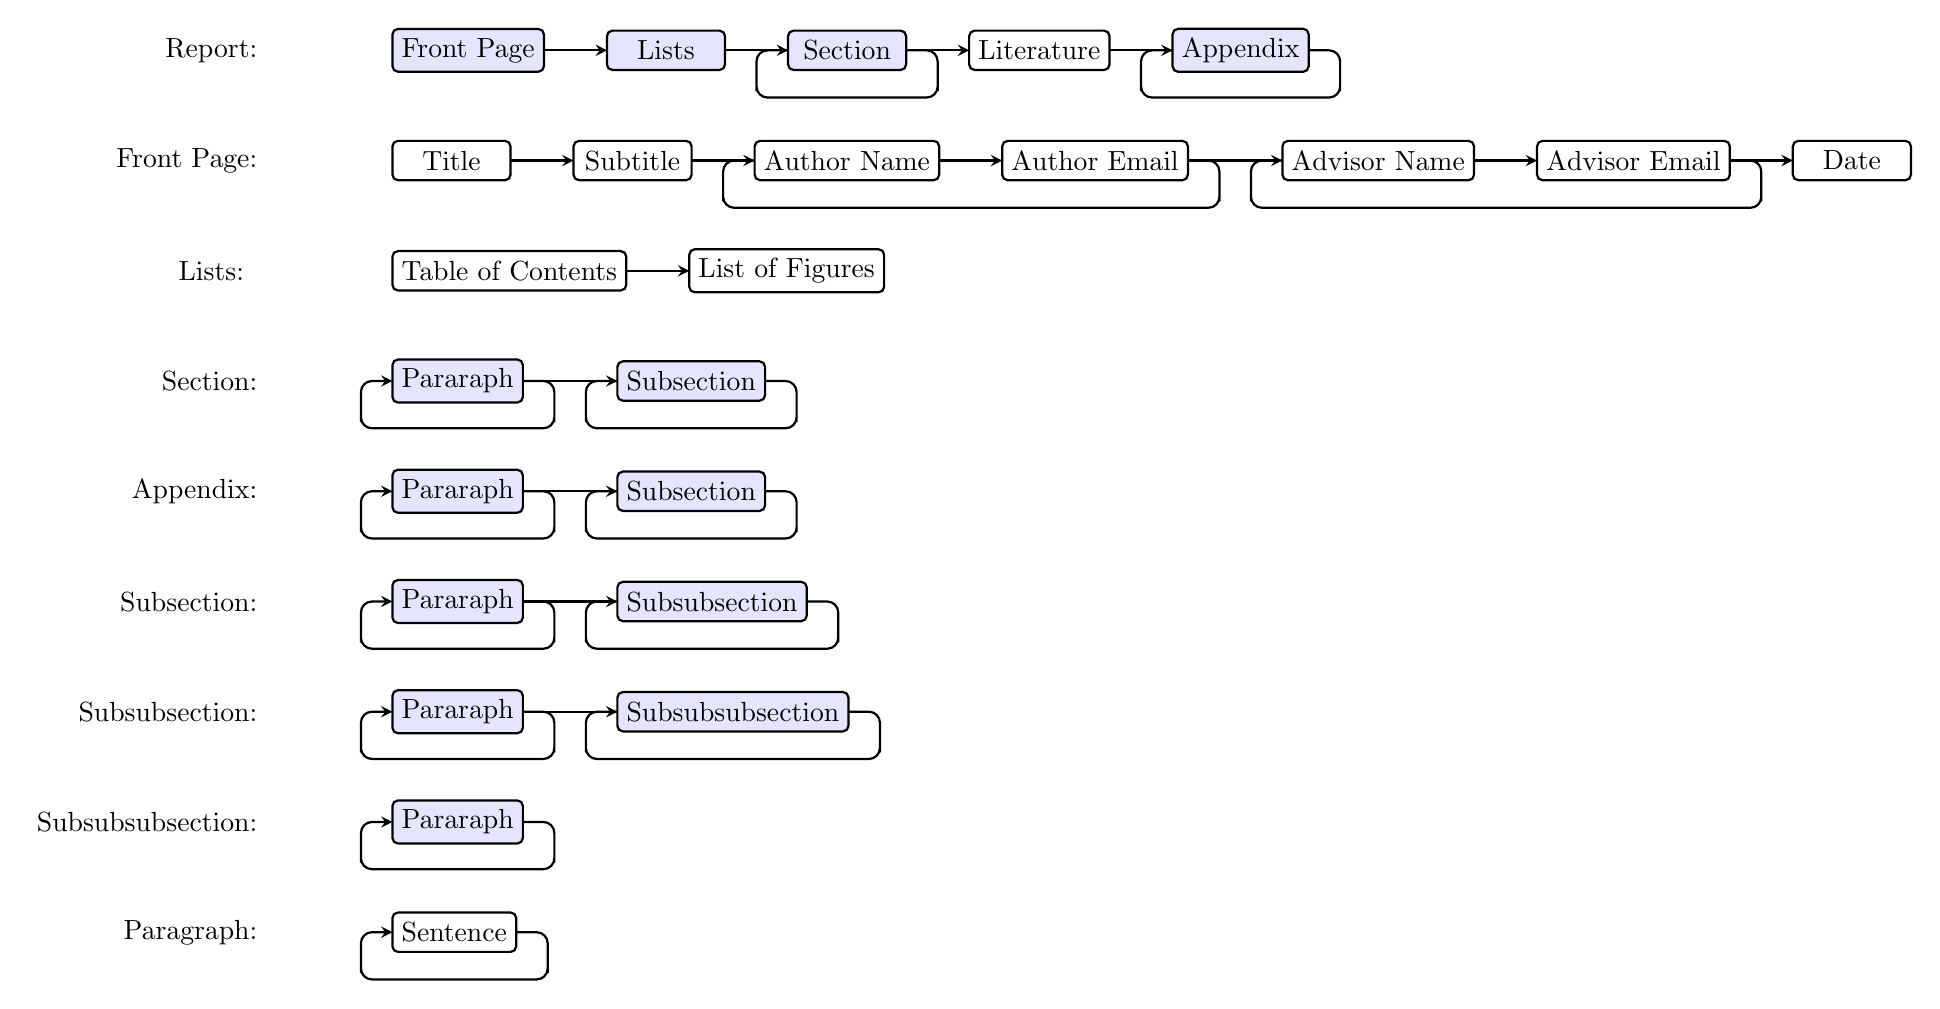
\begin{tikzpicture}[x=1cm, y=-1cm, node distance=0 cm,outer sep = 0pt]
          \newcommand{\textminheight}{5mm}
          \newcommand{\defminwidth}{14mm}
          \newcommand{\defxoffset}{-10mm}
          \newcommand{\spacing}{8mm}
          \newcommand{\loopheight}{6mm}
          
          \tikzstyle{node}=[
            draw,
            rectangle,
            rounded corners=2pt,
            minimum height=\textminheight,
            minimum width=1.5cm,
            fill=blue!10,
            anchor=west,
            thick
          ]
          \tikzstyle{nodet}=[
            draw,
            rectangle,
            rounded corners=2pt,
            minimum height=\textminheight,
            minimum width=1.5cm,
            fill=white!10,
            anchor=west,
            thick
          ]
          \tikzstyle{def}=[
            draw=none,
            minimum height=\textminheight,
            minimum width=\defminwidth,
            anchor=east,
          ]
          \tikzstyle{line} = [thick, rounded corners, draw=black]
          \tikzstyle{arrow} = [thick,->,>=stealth, draw=black]
          
          \coordinate (origo) at (1,1);
          \coordinate (oreport)           at ([xshift=0, yshift=0mm] origo);
          \coordinate (ofront)            at  ([xshift=0, yshift=-1*(\textminheight+\loopheight*1.5)] origo);
          \coordinate (olists)            at  ([xshift=0, yshift=-2*(\textminheight+\loopheight*1.5)] origo);
          \coordinate (osection)          at  ([xshift=0, yshift=-3*(\textminheight+\loopheight*1.5)] origo);
          \coordinate (oappendix)         at  ([xshift=0, yshift=-4*(\textminheight+\loopheight*1.5)] origo);
          \coordinate (osubsection)       at  ([xshift=0, yshift=-5*(\textminheight+\loopheight*1.5)] origo);
          \coordinate (osubsubsection)    at ([xshift=0, yshift=-6*(\textminheight+\loopheight*1.5)] origo);
          \coordinate (osubsubsubsection) at ([xshift=0, yshift=-7*(\textminheight+\loopheight*1.5)] origo);
          \coordinate (oparagraph)        at ([xshift=0, yshift=-8*(\textminheight+\loopheight*1.5)] origo);
          
          % report
          \node[def] (defreport) at ([xshift=\defxoffset] oreport) {Report:};
          \node[node] (report_front) at ([xshift=\defxoffset+\spacing*2] oreport) {Front Page};
          \node[node] (report_lists) at ([xshift=\spacing] report_front.east) {Lists};
          \node[node] (report_section) at ([xshift=\spacing] report_lists.east) {Section};
          \node[nodet] (report_lit) at ([xshift=\spacing] report_section.east) {Literature};
          \node[node] (report_appendix) at ([xshift=\spacing] report_lit.east) {Appendix};
          \draw[arrow] (report_front) -- (report_lists);
          \draw[arrow] (report_lists) -- (report_section);
          \draw[arrow] (report_section) -- (report_lit);
          \draw[arrow] (report_lit) -- (report_appendix);
          \draw[line] (report_section.east) -- ++(\spacing/2,0em) |- ++(0em,-\loopheight) |- ([xshift=-\spacing/2, yshift=-\loopheight] report_section.west) -| ([xshift=-\spacing/2] report_section.west) -- (report_section.west);
          \draw[line] (report_appendix.east) -- ++(\spacing/2,0em) |- ++(0em,-\loopheight) |- ([xshift=-\spacing/2, yshift=-\loopheight] report_appendix.west) -| ([xshift=-\spacing/2] report_appendix.west) -- (report_appendix.west);
          
          % front page
          \node[def] (deffront) at ([xshift=\defxoffset] ofront) {Front Page:};
          \node[nodet] (front_title) at ([xshift=\defxoffset+\spacing*2] ofront) {Title};
          \node[nodet] (front_subtitle) at ([xshift=\spacing] front_title.east) {Subtitle};
          \node[nodet] (front_author_n) at ([xshift=\spacing] front_subtitle.east) {Author Name};
          \node[nodet] (front_author_e) at ([xshift=\spacing] front_author_n.east) {Author Email};
          \node[nodet] (front_advisor_n) at ([xshift=\spacing*1.5] front_author_e.east) {Advisor Name};
          \node[nodet] (front_advisor_e) at ([xshift=\spacing] front_advisor_n.east) {Advisor Email};
          \node[nodet] (front_date) at ([xshift=\spacing] front_advisor_e.east) {Date};
          \draw[arrow] (front_title) -- (front_subtitle);
          \draw[arrow] (front_subtitle) -- (front_author_n);
          \draw[arrow] (front_author_n) -- (front_author_e);
          \draw[arrow] (front_author_e) -- (front_advisor_n);
          \draw[arrow] (front_advisor_n) -- (front_advisor_e);
          \draw[arrow] (front_advisor_e) -- (front_date);
          \draw[line] (front_author_e.east) -- ++(\spacing/2,0em) |- ++(0em,-\loopheight) |- ([xshift=-\spacing/2, yshift=-\loopheight] front_author_n.west) -| ([xshift=-\spacing/2] front_author_n.west) -- (front_author_n.west);
          \draw[line] (front_advisor_e.east) -- ++(\spacing/2,0em) |- ++(0em,-\loopheight) |- ([xshift=-\spacing/2, yshift=-\loopheight] front_advisor_n.west) -| ([xshift=-\spacing/2] front_advisor_n.west) -- (front_advisor_n.west);
          
          % lists
          \node[def] (deflists) at ([xshift=\defxoffset] olists) {Lists:};
          \node[nodet] (lists_toc) at ([xshift=\defxoffset+\spacing*2] olists) {Table of Contents};
          \node[nodet] (lists_lof) at ([xshift=\spacing] lists_toc.east) {List of Figures};
          \draw[arrow] (lists_toc) -- (lists_lof);
          
          % section
          \node[def] (defsection) at ([xshift=\defxoffset] osection) {Section:};
          \node[node] (section_paragraph) at ([xshift=\defxoffset+\spacing*2] osection) {Pararaph};
          \node[node] (section_subsection) at ([xshift=\spacing*1.5] section_paragraph.east) {Subsection};
          \draw[arrow] (section_paragraph) -- (section_subsection);
          \draw[arrow, rounded corners] (section_paragraph.east) -- ++(\spacing/2,0em) |- ++(0em,-\loopheight) |- ([xshift=-\spacing/2, yshift=-\loopheight] section_paragraph.west) -| ([xshift=-\spacing/2] section_paragraph.west) -- (section_paragraph.west);
          \draw[line] (section_subsection.east) -- ++(\spacing/2,0em) |- ++(0em,-\loopheight) |- ([xshift=-\spacing/2, yshift=-\loopheight] section_subsection.west) -| ([xshift=-\spacing/2] section_subsection.west) -- (section_subsection.west);
          
          % appendix
          \node[def] (defappendix) at ([xshift=\defxoffset] oappendix) {Appendix:};
          \node[node] (appendix_paragraph) at ([xshift=\defxoffset+\spacing*2] oappendix) {Pararaph};
          \node[node] (appendix_subsection) at ([xshift=\spacing*1.5] appendix_paragraph.east) {Subsection};
          \draw[arrow] (appendix_paragraph) -- (appendix_subsection);
          \draw[arrow, rounded corners] (appendix_paragraph.east) -- ++(\spacing/2,0em) |- ++(0em,-\loopheight) |- ([xshift=-\spacing/2, yshift=-\loopheight] appendix_paragraph.west) -| ([xshift=-\spacing/2] appendix_paragraph.west) -- (appendix_paragraph.west);
          \draw[line] (appendix_subsection.east) -- ++(\spacing/2,0em) |- ++(0em,-\loopheight) |- ([xshift=-\spacing/2, yshift=-\loopheight] appendix_subsection.west) -| ([xshift=-\spacing/2] appendix_subsection.west) -- (appendix_subsection.west);
          
          % subsection
          \node[def] (defsubsection) at ([xshift=\defxoffset] osubsection) {Subsection:};
          \node[node] (subsection_paragraph) at ([xshift=\defxoffset+\spacing*2] osubsection) {Pararaph};
          \node[node] (subsection_subsubsection) at ([xshift=\spacing*1.5] subsection_paragraph.east) {Subsubsection};
          \draw[arrow] (subsection_paragraph) -- (subsection_subsubsection);
          \draw[arrow, rounded corners] (subsection_paragraph.east) -- ++(\spacing/2,0em) |- ++(0em,-\loopheight) |- ([xshift=-\spacing/2, yshift=-\loopheight] subsection_paragraph.west) -| ([xshift=-\spacing/2] subsection_paragraph.west) -- (subsection_paragraph.west);
          \draw[line] (subsection_subsubsection.east) -- ++(\spacing/2,0em) |- ++(0em,-\loopheight) |- ([xshift=-\spacing/2, yshift=-\loopheight] subsection_subsubsection.west) -| ([xshift=-\spacing/2] subsection_subsubsection.west) -- (subsection_subsubsection.west);
          
          % subsubsection
          \node[def] (defsubsubsection) at ([xshift=\defxoffset] osubsubsection) {Subsubsection:};
          \node[node] (subsubsection_paragraph) at ([xshift=\defxoffset+\spacing*2] osubsubsection) {Pararaph};
          \node[node] (subsubsection_subsubsubsection) at ([xshift=\spacing*1.5] subsubsection_paragraph.east) {Subsubsubsection};
          \draw[arrow] (subsubsection_paragraph) -- (subsubsection_subsubsubsection);
          \draw[arrow, rounded corners] (subsubsection_paragraph.east) -- ++(\spacing/2,0em) |- ++(0em,-\loopheight) |- ([xshift=-\spacing/2, yshift=-\loopheight] subsubsection_paragraph.west) -| ([xshift=-\spacing/2] subsubsection_paragraph.west) -- (subsubsection_paragraph.west);
          \draw[line] (subsubsection_subsubsubsection.east) -- ++(\spacing/2,0em) |- ++(0em,-\loopheight) |- ([xshift=-\spacing/2, yshift=-\loopheight] subsubsection_subsubsubsection.west) -| ([xshift=-\spacing/2] subsubsection_subsubsubsection.west) -- (subsubsection_subsubsubsection.west);
          
          % subsubsubsection
          \node[def] (defsubsubsubsection) at ([xshift=\defxoffset] osubsubsubsection) {Subsubsubsection:};
          \node[node] (subsubsubsection_paragraph) at ([xshift=\defxoffset+\spacing*2] osubsubsubsection) {Pararaph};
          \draw[arrow, rounded corners] (subsubsubsection_paragraph.east) -- ++(\spacing/2,0em) |- ++(0em,-\loopheight) |- ([xshift=-\spacing/2, yshift=-\loopheight] subsubsubsection_paragraph.west) -| ([xshift=-\spacing/2] subsubsubsection_paragraph.west) -- (subsubsubsection_paragraph.west);
          
          % paragraph
          \node[def] (defparagraph) at ([xshift=\defxoffset] oparagraph) {Paragraph:};
          \node[nodet] (paragraph_sentence) at ([xshift=\defxoffset+\spacing*2] oparagraph) {Sentence};
          \draw[arrow, rounded corners] (paragraph_sentence.east) -- ++(\spacing/2,0em) |- ++(0em,-\loopheight) |- ([xshift=-\spacing/2, yshift=-\loopheight] paragraph_sentence.west) -| ([xshift=-\spacing/2] paragraph_sentence.west) -- (paragraph_sentence.west);
        \end{tikzpicture}
      }
    \end{adjustbox}
  \caption{\label{fig:firststeps:process:bnf} Railroad BNF of a typical report structure.}
\end{figure}

% differences in opinion
But how do you come up with that tree structure; the \textsl{right} tree structure? People tend to prefer one of two strategies, and despise the other. I have seen both work for people who chose it of their own free will.

% first strat
The first strategy is to first get something (anything, really) down "on paper", and then iterate and keep on iterating until the end result is good. I am not a fan of this approach. Generally, it requires a lot of writing experience to succeed, the overhead of repeated iterations is high, and the iterations usually end up being cut short before a good result has been reached.

% second strat
The second strategy is to go top-down by growing the tree from the root. Only after understanding the final structure of a node (at a single level of depth) are you allowed to dig into a child node. Note that this allows you to go deep in some parts of the report while having little understanding of others.

% second strat: mindset
That implies a process of considering the topic of the node and all that came before it, and deciding:
\begin{enumerate}
  \item Which key points have to be covered?
  \item Which pseudo points are needed to support these?
  \item What is the best way of serializing the coverage of all of these points?
  \item How can that sequence be broken down into themes?
\end{enumerate}
These themes are your subsections. Often it makes sense to consider naming conventions that transcends a single subtree to bring some consistency to the report.

% second strat: tool
Large reports can become hard to navigate and conclusions on the exact contents of som subsection may escape memory. One way of dealing with this is to write down pre and post conditions for individual (sub*)sections. This works particularly well in \LaTeX\ where you have comments:

\begin{minted}[breaklines]{latex}
\subsection{Publish Subscribe Substrates}
\label{sec:analysis:transport:pubsub}
% pre: It has been established that a transport is needed for moving streaming data from backend to front-end at a rate of 10-20Hz. Parameters for evaluation: [latency, throughput, robustness, inspection].
% post: A clear definition of the pros and cons of using pubsub for this purpose.
\end{minted}

\section{Working Document}

It is a good practice in a project to quickly establish a working report document. That gives you a natural area to drop notes about your design choices (so that you can later remember why you did things the way you ended up doing them) and have a low bar for writing on your report should you suddenly feel inspired. You can organically structure the report as your perception of its shape matures, and -- if frequently visited -- it will keep your mind fixed on which details matter for the end-goal of producing the report handin.

This document represents a dissertation. In the beginning of it you are likely to have a central thesis, or maybe a number of theses that you wish to explore. The starting point is what you came up with in your project description (see section \ref{sec:projectdesc}). I recommend filling out the contents of each section as you go through the corresponding phases of the project. That way the details are still sharp in your mind, it is easy to make sure that you don't miss anything, and you don't end up with a whole lot of report work at the end.

\section{Report Structure}

\idx{Report structure} The following is a good starting point for the structure of most reports. If you end up with \textsl{interesting} parts of your implementation then you can add an \textdesc{Implementation} section. However, we do -- especially at the MSc level -- expect you to be able to write code, and we generally don't care about you choosing a \keywordname{for} loop over a \keywordname{while} loop.

\begin{enumerate}
  \descitem{Table of Contents}
  \descitem{List of Figures}
  \descitem{Introduction} 
    \begin{enumerate}[label*=\arabic*.]
      \descitem{Problem}
      \descitem{Approach}
    \end{enumerate}
  \descitem{Process}
  \descitem{Related Work}
  \descitem{Analysis}
  \descitem{Design}
  \descitem{Evaluation}
  \descitem{Discussion}
  \descitem{Future Work}
  \descitem{Hindsight}
  \descitem{Conclusion}
  \descitem{Literature}
  \descitem{Appendix}
\end{enumerate}

%%%%%%%%%%%%%%%%%%%%%%%%%%%%%%%%%%%%%%%%%%%%%%%%%%%%%%%%%%%%%%%%%%%%%%%%%%%%%%%%
%%%%%%%%%%%%%%%%%%%%%%%%%%%%%%%%%%%%%%%%%%%%%%%%%%%%%%%%%%%%% The Art of Writing
\chapter{The Art of Writing}
\label{chap:artofwriting}

\begin{inspiration}{Stephen King\idxx{King, Stephen}{Stephen King}\cite{king2000writing}}
  ``
    \textsl{To write is human, to edit is divine.}
  ''
\end{inspiration}
\begin{inspiration}{David McCullough\idxx{McCullough, David}{David McCullough}\cite{McCullough2002}}
  ``
    \textsl{Writing is thinking. To write well is to think clearly. That's why it's so hard.}
  ''
\end{inspiration}

% writing is a directed effort
Writing requires directed effort that considers what comes later in addition to what came before. Very few people can produce good text without laying a plan. The rest of us will have spend -- seemingly unproductive -- time considering what exactly it is we want to convey, how that fits into a narrative and which words to use in order to best express that narrative.

\section{Commandments}

\idx{Commandments}
\begin{enumerate}
  \descitem{Make the Effort} \idx{Effort}
    As with pretty much else in life, if you want to excel at writing you need to put in significant amounts of focused work and active considerations about the nature of what makes a text good. Take pride in your work.
  \descitem{It Has to Make Sense}
    Above all else, what you do (and write) has to make sense. This should be your guiding light throughout the entire project. Much can be excused as long as the it is done for the right reasons. While this is used to balance learning objectives according to the individual project, in cannot completely remove a learning objective.
  \descitem{Give and Take Credit} \idx{Credit}
    In order to evaluate the contribution of a text it is necessary to know which parts the author has been responsible for contributing. If some insight, term or similar is original, then credit should be given to the author. If not, then credit should be given to the original authors (e.g., through a citation) and credit should be given to the author for citing them. It is bad practice to leave credit unclear, and it erodes overall confidence in the text itself. Therefore, always make sure that you give credit where it is needed, and take credit where you can.
  \descitem{Best Practices are Fallacies} \idx{Best practices}
    While it is a good practice to explore best practices, real projects never seem to be quite that simple. Best practices are based on typical situations, and it is thus a good practice to be critical towards them. You will likely have to violate\idx{Fallacy} one or two of them.
  \descitem{Do not Underestimate Experimental Evaluation} \idxx{Evaluation!Experimental}{Experimental evaluation}
    When working on something of experimental nature it is hard to assess the time to completion. Before beginning the work it is harder. Does all the needed experimental tooling already exists, or do you need to construct parts of it yourself? How many repetitions are necessary to get trustworthy results? How much time is needed to conduct the experiments? Which kinds of post processing of results are needed to reach the relevant insights?
    However long you think it is going to take, it is going to take longer. In part because things are going to go wrong, and you might realize that your design needs to change. For that to even be a possibility, you need to start experimental work early. A good rule of thumb is to take the time you expect it to take, and multiply it by $\pi$.
  \descitem{Respect your Audience} \idx{Audience}
    You are writing a report because you expect someone to read it. Knowing who that someone is is key to understanding what is necessary in order to convey your subject. You can expect your reader to have an IT-related background and at least an MSc. Also, you should expect the reader to print your report on A4 paper. A consequence of this is that you cannot rely on the reader zooming in to read certain parts of a figure.
    \begin{inspiration}[0.82]{Rupert Giles\idxx{Giles, Rupert}{Rupert Giles}\cite{buffy_s1e8}}
  ``
    \textsl{Smell is the most powerful trigger to the memory there is. A certain flower or a whiff of smoke can bring up experiences long forgotten. Books smell musty and rich. The knowledge gained from a computer is \ldots\ it has no texture, no context. It's there and then it's gone. If it's to last, then the getting of knowledge should be tangible. It should be, um, smelly.}
  ''
\end{inspiration}
  \descitem{One sentence One message}
    Rarely is anything achieved by having a single sentence deliver more than a single message. Often, readability is affected negatively. A sequence of short messages, each progressing the narrative towards a point is a simple way of ensuring a concise and readable language. It takes considerable effort to shoehorn multiple messages into a single sentence without negatively affecting readability.
  \descitem{A Text Should Be Self-Contained}
    A text (e.g., a paragraph) may refer to other resources like sections, citations, appendices or floats (figures and tables), but the reader should not need to follow any of these to read the text. So, when referring to a figure\idx{Figure} make sure to highlight what you would get out of looking at it. The reader then has a \textsl{choice} of looking at the figure. In much the same way, when looking at the figure the reader should not have to look for a reference in the text for that figure in order to understand how to read it. Instead these details should be covered by a legend or the figures label.
  \descitem{The Specific-Generic Spectrum} \idx{Specific-generic spectrum}% Can we make this statement more specific to a degree where it is as wide as possible without becoming untrue for some cases?
    Most statements has (at least one) inherent specificity. That is, what it expresses fits on a scale from specific to generic. If a statement is too generic then part of it is untrue. That is obviously problematic. If a statement is too specific then it doesn't express the full gamut of the underlying mechanics. That is less-obviously problematic. Perhaps it doesn't need to be covered to make your point, but it is makes it unclear whether you actually understand those implications. So, make every statement specific to a degree where it is as wide as possible without becoming untrue for any case.
  \descitem{Make the Argument Explicit} \idx{Argument}
    When providing an argument, do not rely on the reader to fold out steps that you consider implicit. The reader may have other standards for what is implicit, or have a different cultural background where those steps are not obvious. Also, this is an opportunity to show that you can construct a line of reasoning, and that opportunity should be grabbed.
  \descitem{Remember the Context} \idx{Context}
    Everything communicated is expressed in some context. Key aspects of this context are necessary to correctly decipher the communication. Be aware of these aspects and make sure that they are shared with the reader. For instance, the word \quoted{technical} can be rooted in software, but could also be legal or mechanical. I assume that people from legal also refer to the technical aspects, but have a fairly different interpretation of what that means.
\end{enumerate}

\section{Coverage}

% intro: when does this apply?
When we have several -- potentially interdependent -- decisions to make we say that there is a \textsl{decision space}\idx{Decision space} to cover. It is critical that it is obvious to the reader that the entire decision space is being covered. We say that we are \textsl{going for coverage}\idx{Coverage}. To do that, whenever we are faced with a choice, we need to consider all the options, and dive into those that cannot be ruled out. This way we prune\idxx{Search tree!Pruning}{Pruning} the search tree\idx{Search tree}. If two parts (e.g., aspects) of the decision space interact, then we need to treat them as equals and consider their interactions.

\begin{figure}[tbp]
  \begin{center}
    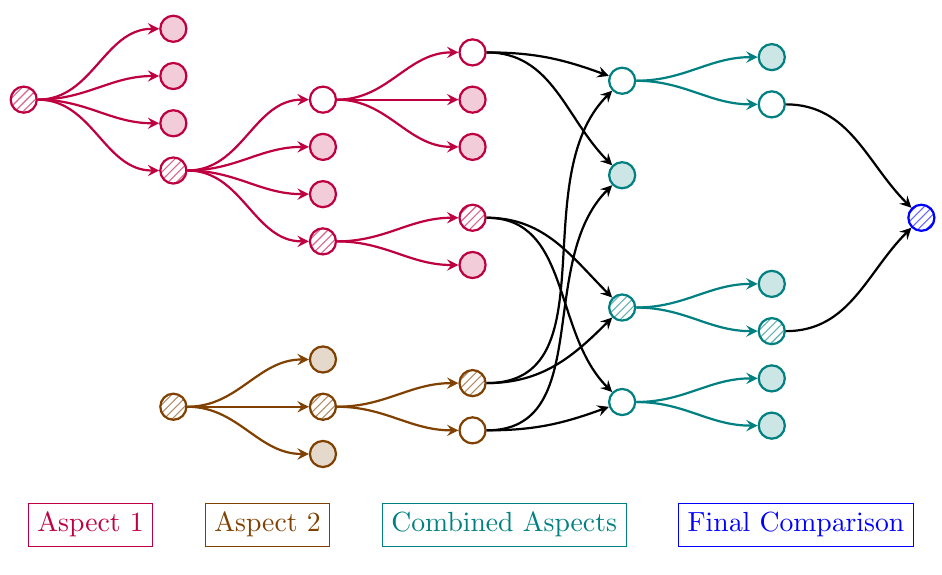
\begin{tikzpicture}
      \newcommand{\yspacing}[0]{6mm}
      \newcommand{\xspacing}[0]{19mm}
      \newcommand{\legendxspacing}[0]{6.5mm}
      \newcommand{\colorAspectI}[0]{purple}
      \newcommand{\colorAspectII}[0]{orange!50!black}
      \newcommand{\colorAspectsCombinedI}[0]{teal}
      \newcommand{\colorAspectsCombinedII}[0]{blue}
      \newcommand{\colorAspectIdead}[0]{\colorAspectI!20}
      \newcommand{\colorAspectIIdead}[0]{\colorAspectII!20}
      \newcommand{\colorAspectsCombinedIdead}[0]{\colorAspectsCombinedI!20}
      \newcommand{\colorAspectsCombinedIIdead}[0]{\colorAspectsCombinedII!20}
      
      \tikzstyle{edge} = [thick,->,>=stealth,draw=black]
      \tikzstyle{edgeAspectI} = [edge,draw=\colorAspectI]
      \tikzstyle{edgeAspectII} = [edge,draw=\colorAspectII]
      \tikzstyle{edgeAspectsCombinedI} = [edge,draw=\colorAspectsCombinedI]
      \tikzstyle{edgeAspectsCombinedII} = [edge,draw=\colorAspectsCombinedII]
      
      \tikzstyle{node}=[
        overlay,
        circle,
        draw=purple,
        anchor=center,
        thick,
        minimum size=1,
      ]
      \tikzstyle{nodeAspectI}=[
        node,
        draw=\colorAspectI,
      ]
      \tikzstyle{nodeAspectII}=[
        node,
        draw=\colorAspectII,
      ]
      \tikzstyle{nodeAspectsCombinedI}=[
        node,
        draw=\colorAspectsCombinedI,
      ]
      \tikzstyle{nodeAspectsCombinedII}=[
        node,
        draw=\colorAspectsCombinedII,
      ]
      
      \tikzstyle{chosenAspectI}=[
        pattern=north east lines,
        pattern color=\colorAspectI!60,
        even odd rule,
      ]
      \tikzstyle{chosenAspectII}=[
        pattern=north east lines,
        pattern color=\colorAspectII!60,
        even odd rule,
      ]
      \tikzstyle{chosenAspectsCombinedI}=[
        pattern=north east lines,
        pattern color=\colorAspectsCombinedI!60,
        even odd rule,
      ]
      \tikzstyle{chosenAspectsCombinedII}=[
        pattern=north east lines,
        pattern color=\colorAspectsCombinedII!60,
        even odd rule,
      ]
      
      % https://tex.stackexchange.com/questions/141378/path-following-color-gradient-in-tikz
      \tikzset{gradient/.style n args={3}{
        postaction={
          decorate,
          decoration={
            markings,
            mark=between positions 0 and \pgfdecoratedpathlength step 0.5pt with {
              \pgfmathsetmacro\myval{multiply(
                  divide(
                  \pgfkeysvalueof{/pgf/decoration/mark info/distance from start}, \pgfdecoratedpathlength
                  ),
                  100
              )};
              \pgfsetfillcolor{#3!\myval!#2};
              \pgfpathcircle{\pgfpointorigin}{#1};
              \pgfusepath{fill};
            }
          }
        }
      }}
      
      % nodes and edges
      {
        {
          \node[nodeAspectI,chosenAspectI] (n1) at (0,0) {};
          
          \node[nodeAspectI,fill=\colorAspectIdead] (n11) at ([yshift= 1.5*\yspacing, xshift=\xspacing] n1) {};
          \node[nodeAspectI,fill=\colorAspectIdead] (n12) at ([yshift= 0.5*\yspacing, xshift=\xspacing] n1) {};
          \node[nodeAspectI,fill=\colorAspectIdead] (n13) at ([yshift=-0.5*\yspacing, xshift=\xspacing] n1) {};
          \node[nodeAspectI,chosenAspectI] (n14) at ([yshift=-1.5*\yspacing, xshift=\xspacing] n1) {};
          \draw[edgeAspectI] (n1) to [out=0,in=180] (n11);
          \draw[edgeAspectI] (n1) to [out=0,in=180] (n12);
          \draw[edgeAspectI] (n1) to [out=0,in=180] (n13);
          \draw[edgeAspectI] (n1) to [out=0,in=180] (n14);
          
          \node[nodeAspectI] (n141) at ([yshift= 1.5*\yspacing, xshift=\xspacing] n14) {};
          \node[nodeAspectI,fill=\colorAspectIdead] (n142) at ([yshift= 0.5*\yspacing, xshift=\xspacing] n14) {};
          \node[nodeAspectI,fill=\colorAspectIdead] (n143) at ([yshift=-0.5*\yspacing, xshift=\xspacing] n14) {};
          \node[nodeAspectI,chosenAspectI] (n144) at ([yshift=-1.5*\yspacing, xshift=\xspacing] n14) {};
          \draw[edgeAspectI] (n14) to [out=0,in=180] (n141);
          \draw[edgeAspectI] (n14) to [out=0,in=180] (n142);
          \draw[edgeAspectI] (n14) to [out=0,in=180] (n143);
          \draw[edgeAspectI] (n14) to [out=0,in=180] (n144);
          
          \node[nodeAspectI] (n1411) at ([yshift= 1*\yspacing, xshift=\xspacing] n141) {};
          \node[nodeAspectI,fill=\colorAspectIdead] (n1412) at ([yshift= 0*\yspacing, xshift=\xspacing] n141) {};
          \node[nodeAspectI,fill=\colorAspectIdead] (n1413) at ([yshift=-1*\yspacing, xshift=\xspacing] n141) {};
          \node[nodeAspectI,chosenAspectI] (n1441) at ([yshift= 0.5*\yspacing, xshift=\xspacing] n144) {};
          \node[nodeAspectI,fill=\colorAspectIdead] (n1442) at ([yshift=-0.5*\yspacing, xshift=\xspacing] n144) {};
          \draw[edgeAspectI] (n141) to [out=0,in=180] (n1411);
          \draw[edgeAspectI] (n141) to [out=0,in=180] (n1412);
          \draw[edgeAspectI] (n141) to [out=0,in=180] (n1413);
          \draw[edgeAspectI] (n144) to [out=0,in=180] (n1441);
          \draw[edgeAspectI] (n144) to [out=0,in=180] (n1442);
        }
        
        {
          \node[nodeAspectII,chosenAspectII] (n221) at ([yshift=-2.5*\yspacing, xshift=0] n1442) {};
          \node[nodeAspectII] (n222) at ([yshift=-3.5*\yspacing, xshift=0] n1442) {};
          
          \node[nodeAspectII,chosenAspectII] (n22) at ([yshift=-0.5*\yspacing, xshift=-\xspacing] n221) {};
          \node[nodeAspectII,fill=\colorAspectIIdead] (n21) at ([yshift= 1*\yspacing, xshift=0] n22) {};
          \node[nodeAspectII,fill=\colorAspectIIdead] (n23) at ([yshift=-1*\yspacing, xshift=0] n22) {};
          \draw[edgeAspectII] (n22) to [out=0,in=180] (n221);
          \draw[edgeAspectII] (n22) to [out=0,in=180] (n222);
          
          \node[nodeAspectII,chosenAspectII] (n2) at ([yshift=0, xshift=-\xspacing] n22) {};
          \draw[edgeAspectII] (n2) to [out=0,in=180] (n21);
          \draw[edgeAspectII] (n2) to [out=0,in=180] (n22);
          \draw[edgeAspectII] (n2) to [out=0,in=180] (n23);
        }
        
        % merged graph
        {
          \coordinate (m1) at ($(n1411)!0.2!(n222)$);
          \coordinate (m2) at ($(n1411)!0.8!(n222)$);
          
          \node[nodeAspectsCombinedI] (m1n1) at ([yshift= 1*\yspacing, xshift=\xspacing] m1) {};
          \node[nodeAspectsCombinedI,fill=\colorAspectsCombinedIdead] (m1n2) at ([yshift=-1*\yspacing, xshift=\xspacing] m1) {};
          \node[nodeAspectsCombinedI,chosenAspectsCombinedI] (m2n1) at ([yshift= 1*\yspacing, xshift=\xspacing] m2) {};
          \node[nodeAspectsCombinedI] (m2n2) at ([yshift=-1*\yspacing, xshift=\xspacing] m2) {};
          \draw[edge] (n1411) to [out=0,in=160] (m1n1);
          \draw[edge] (n1411) to [out=0,in=135] (m1n2);
          \draw[edge] (n1441) to [out=0,in=135] (m2n1);
          \draw[edge] (n1441) to [out=0,in=135] (m2n2);
          \draw[edge] (n221) to [out=0,in=225] (m1n1);
          \draw[edge] (n222) to [out=0,in=225] (m1n2);
          \draw[edge] (n221) to [out=0,in=225] (m2n1);
          \draw[edge] (n222) to [out=0,in=200] (m2n2);
          
          \node[nodeAspectsCombinedI,fill=\colorAspectsCombinedIdead] (m1n11) at ([yshift= 0.5*\yspacing, xshift=\xspacing] m1n1) {};
          \node[nodeAspectsCombinedI] (m1n12) at ([yshift=-0.5*\yspacing, xshift=\xspacing] m1n1) {};
          \draw[edgeAspectsCombinedI] (m1n1) to [out=0,in=180] (m1n11);
          \draw[edgeAspectsCombinedI] (m1n1) to [out=0,in=180] (m1n12);
          
          \node[nodeAspectsCombinedI,fill=\colorAspectsCombinedIdead] (m2n11) at ([yshift= 0.5*\yspacing, xshift=\xspacing] m2n1) {};
          \node[nodeAspectsCombinedI,chosenAspectsCombinedI] (m2n12) at ([yshift=-0.5*\yspacing, xshift=\xspacing] m2n1) {};
          \draw[edgeAspectsCombinedI] (m2n1) to [out=0,in=180] (m2n11);
          \draw[edgeAspectsCombinedI] (m2n1) to [out=0,in=180] (m2n12);
          
          \node[nodeAspectsCombinedI,fill=\colorAspectsCombinedIdead] (m2n21) at ([yshift= 0.5*\yspacing, xshift=\xspacing] m2n2) {};
          \node[nodeAspectsCombinedI,fill=\colorAspectsCombinedIdead] (m2n22) at ([yshift=-0.5*\yspacing, xshift=\xspacing] m2n2) {};
          \draw[edgeAspectsCombinedI] (m2n2) to [out=0,in=180] (m2n21);
          \draw[edgeAspectsCombinedI] (m2n2) to [out=0,in=180] (m2n22);
        }
        
        {
          \coordinate (l1) at ($(m1n12)!0.5!(m2n12)$);
          \node[nodeAspectsCombinedII,chosenAspectsCombinedII] (l1n1) at ([yshift=0, xshift=\xspacing] l1) {};
          \draw[edge] (m1n12) to [out=0,in=135] (l1n1);
          \draw[edge] (m2n12) to [out=0,in=225] (l1n1);
        }
      }
      
      % legend
      {
        \coordinate (legend) at ([yshift=-54mm, xshift=-6mm] n1);
        
        \node[rectangle,anchor=west,draw=\colorAspectI,text=\colorAspectI] (legendAspectI) at ([xshift=\legendxspacing] legend) {Aspect 1};
        \node[rectangle,anchor=west,draw=\colorAspectII,text=\colorAspectII] (legendAspectII) at ([xshift=\legendxspacing] legendAspectI.east) {Aspect 2};
        \node[rectangle,anchor=west,draw=\colorAspectsCombinedI,text=\colorAspectsCombinedI] (legendAspectsCombinedI) at ([xshift=\legendxspacing] legendAspectII.east) {Combined Aspects};
        \node[rectangle,anchor=west,draw=\colorAspectsCombinedII,text=\colorAspectsCombinedII] (legendAspectsCombinedII) at ([xshift=\legendxspacing] legendAspectsCombinedI.east) {Final Comparison};
      }
    \end{tikzpicture}
  \end{center}
  \caption[Pruning the coverage DAG]{Pruning the coverage DAG. Filled nodes represent dead ends, and nodes with a pattern fill represents the chosen path.}
  \label{fig:writing:coverage}
\end{figure}

% approach: go through figure (aspect 1, 1/4 viable options, 2/4 viable options, aspect 2, 1/3 viable options, 2/2 viable options, 3/4 combinations viable, from these we end up with two viable options that are then compared)
Figure \ref{fig:writing:coverage} visually illustrates an approach for making sure that everything gets covered. In this particular scenario, there are two aspects to consider. For the first aspect a number of choices has to be made. The first can be split into four different options. By evaluating these we find that only the last one could be viable. There is no need to consider the dead ends, but given the last option, another choice appears, of which the first and the last option could be viable. We need to follow both of these. Each of them are associated with a new choice with multiple potential options. We end up with two potential paths through this decision tree. Likewise, the second aspect ends up with two potential paths. We now need to combine these. We do by considering every combination of these. Of the for combinations one turns out to be a dead end. For each of the remaining three potential paths there is a last choice, and that leaves two potentially viable paths. A final comparison is made and a winning path is chosen. This path represent the set of choices that went into best path through the entire space, and these are the choices we continue with.

% serialize to text
This example contains a significant amount of complexity\idx{Complexity}. Visually, it is easy to get an overview of, but the text may end up taking 10+ pages. And then it can be hard to keep track. To help the reader you should consider how this should be serialized\idx{Serialization} and mapped to sections, subsections, paragraphs and even sentences. You may even wish to add something like figure \ref{fig:writing:coverage} as an index. If you have space for it, consider expanding each node to include a headline.

\section{Pieces}

\subsection{Definitions}

\subsection{Floats}

% intro: what, examples (figure, table, code listing), refs are necessary
\idx{Floats} A float is a piece of the report that you allow the layouter to place on your behalf. You don't have to care about it being broken up across multiple pages and you get a number that you can use to refer to it through. This is beneficial when you need to refer to it from multiple places in the document. In \LaTeX\idxx{LaTeX@\LaTeX}{\LaTeX}, there are a number of predefined float types (figure, table and code listing springs to mind), and you can define your own. The floats are also presented with a caption and stand out from the normal text.

% refs and context
No matter where the float ends up, you will have to refer to it by number\idxx{Floats!Referencing}{Referencing floats}. The text should always be written in such a manner that it is optional to look at the float. You must explicitly point out what you want the reader to take away from it. In the same way, the floats should make sense without locating the text that refers to them.

% preference
There are different schools of thought with regards to which kinds to floats\idxx{Floats!Types of}{Types of floats} to use. If you have a lot of figures and tables, it might make sense to use these environments so that they end up categorized in a list of figures and a list of tables. Typically, I prefer to use figures for everything. This solves the issue where you have to turn a lot of pages to figure out if you need to go forward or backward in order to find a particular float.

% example
Usually, floats works best when they are allowed to be placed\idxx{Floats!Placement of}{Placement of floats} at the top of a page, the bottom of a page and to fill up a whole page. In \LaTeX, this is accomplished this way:
\begin{minted}[breaklines]{latex}
\begin{figure}[tbp]
  \ldots
  \caption{Description of figure.}
  \label{fig:art:floats}
\end{figure}
\end{minted}

% short captions
Sometimes the caption\idxx{Floats!Caption}{Caption} will naturally take up more space than fits nicely into an entry into the list of figures. The solution is to add a shorter, abbreviated, version that can be used for this purpose. That can be done like this:
\begin{minted}[breaklines]{latex}
\caption[Short caption]{Long caption}
\end{minted}

% landscape mode
At times, a figure may be too complex to be readable in normal (i.e., portrait\idx{Portrait}) orientation\idx{Orientation}. In \LaTeX\ it is easy to scale and rotate elements. To put the contents of a figure in landscape\idx{Landscape} mode use something like this:
\begin{minted}[breaklines]{latex}
\begin{figure}[tbp]
  \begin{center}
    \scalebox{0.7}{
      \rotatebox{90}{
        \ldots
      }
    }
  \end{center}
  \caption{Description of figure that is rotated and scaled.}
  \label{fig:art:floats:landscape}
\end{figure}
\end{minted}

\subsection{Inline Enumerations}

When presenting a choice, we may want to list the consequences of that choice. Similarly, when reasoning about something, we may want to list a number of premises that all hold. We could use bullet points, but that breaks up the paragraph, and thus the flow. Figure \ref{fig:art:pieces:inlineenum:bnf} formalizes an inline enumeration construct that preserves the flow of the text. Here, \textsl{\$text} should be replaced by some text, and \textsl{\$num} by increasing numbers (I prefer lowercase roman numerals). The following is a concrete example of its use.

% example
\begin{center}
  \begin{minipage}{0.9\textwidth}
    \quoted{For the service to stay available we need (i) robust access to the DBMS, (ii) support for hot updates, and (iii) enough processing power to handle requests from both this service and the periodic backup service.}
  \end{minipage}
\end{center}

\begin{figure}
    \centering
      \scalebox{0.7}{
        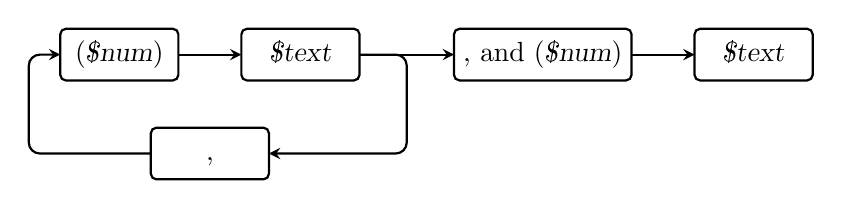
\begin{tikzpicture}[x=1cm, y=-1cm, node distance=0 cm,outer sep = 0pt]
          \newcommand{\textminheight}{5mm}
          \newcommand{\defminwidth}{14mm}
          \newcommand{\defxoffset}{-10mm}
          \newcommand{\spacing}{8mm}
          \newcommand{\loopheight}{6mm}
          
          \tikzstyle{nodet}=[
            draw,
            rectangle,
            rounded corners=2pt,
            minimum height=\textminheight,
            minimum width=1.5cm,
            fill=white!10,
            anchor=west,
            thick
          ]
          \tikzstyle{def}=[
            draw=none,
            minimum height=\textminheight,
            minimum width=\defminwidth,
            anchor=east,
          ]
          \tikzstyle{line} = [thick, rounded corners, draw=black]
          \tikzstyle{arrow} = [thick,->,>=stealth, draw=black]
          
          \coordinate (origo) at (1,1);
          
          % front page
          \node[nodet] (first) at ([xshift=\spacing] origo) {\strut(\textsl{\$num})};
          \node[nodet] (ftext) at ([xshift=\spacing] first.east) {\strut\textsl{\$text}};
          \node[nodet] (last) at ([xshift=\spacing*1.5] ftext.east) {\strut, and (\textsl{\$num})};
          \node[nodet] (ltext) at ([xshift=\spacing] last.east) {\strut\textsl{\$text}};
          
          \node[nodet,anchor=north] (comma) at ([xshift=\spacing/2, yshift=-\loopheight] first.south east) {\strut,};
          
          \draw[arrow] (first) -- (ftext);
          \draw[arrow] (ftext) -- (last);
          \draw[arrow] (last) -- (ltext);
          \draw[arrow, rounded corners] (ftext.east) -- ++(\spacing*1.5/2,0em) |- ++(0em,-\loopheight) |- (comma.east);
          \draw[arrow, rounded corners] (comma.west) -| ([xshift=-\spacing/2] first.west) -- (first.west);
          
        \end{tikzpicture}
      }
  \caption{\label{fig:art:pieces:inlineenum:bnf} Railroad BNF of an inline enumeration.}
\end{figure}

\subsection{Citations}

% why we cite
Each statement we make represent some thoughts. If those thoughts are yours, then you should get credit\idx{Credit} for them. If they are not, then you need to \textsl{give} credit. Otherwise, you will be stealing their work. Conveniently, this mechanism also allows you to not build up your argument from zero. Zero being the level that is generally accepted as truth amongst your peers.

\begin{inspiration}{Isaac Newton\idxx{Newton, Isaac}{Isaac Newton}\cite{Solr-dc-9792}}
  ``
    \textsl{If I have seen further it is by standing on the shoulders of Giants.}
  ''
\end{inspiration}

% when we cite
Every statement must be mapped to an owner. If a statement is not explicitly mapped to someone else, then you are the owner and it is your responsibility to argue for its correctness. If the owner is someone else, then credit need to be given. This is where we use citations. It is, however, still your responsibility to consider the credibility of the source, and to make sure that the full context of the source material is applicable in the situation where you cite it.

% how we cite
There are a number of ways to cite:
\begin{enumerate}
  \item Adding a reference to a concept (e.g., an abbreviation). It is rarely done, and is often better accomplished through a footnote (e.g., with a link). This is done by adding the reference just after the mention of the concept:
    \\
    \mintinline{latex}{The ACM\cite{acm} publishes many articles.}
  \item \label{enum:writing:citations:support} Adding a reference in support of a statement. This is done by adding the reference at the end of the statement (before the period):
    \\
    \mintinline{latex}{The Earth is flat\cite{source}.}
  \item  \label{enum:writing:citations:natural} Natural references. This is done by putting the reference in place of a person:
    \\
    \mintinline{latex}{According to \cite{source} the Earth is flat.}
\end{enumerate}
I usually prefer \ref{enum:writing:citations:support} over \ref{enum:writing:citations:natural} due to its compactness and the separation between message and documentation. It allows me -- as a reader -- to not pay attention to the references, and yet they are still around should I need them. Multiple references can also be given:
\begin{minted}{latex}
A number of the surveyed papers conclude that the Earth is
flat\cite{paper1,paper13,paper16}.
\end{minted}

% what can be cited
Anything can be cited, but all citations are not equally useful. A citation is a reference. It allows the reader to look up the source of the information, verify that it says what you say it says, and evaluate how trustworthy it is. For this to work, it needs to be available to you. Ideally it should be published and without any form of access restriction. But you may have to refer to things that simply don't have that property. Many research papers are paywalled\idx{Paywall}. That is a step down. Maybe some document is published internally in some organization, but still necessary for documenting the decisions you have made. That is worse, but some people can still follow it. It could also be an insight that you received through a private\idx{Private correspondence} correspondence. That is pretty bad, but it can still be verified if you write who was at the other end of that correspondence. And if this insight way key to your project, then you need a way to refer to it.

\section{Questions}

\begin{itemize}
  \descitem{From a scientific point of view -- why does it matter?}
  \descitem{What is the underlying fundamental mechanism?}
\end{itemize}

\section{Anti-Patterns}

\subsection{Use-Before-Definition}

One of the more frustrating experiences of a reader is to read a text that refers to concepts or notions that have not been introduced. Another is when the text later on defines that thing. This is the wrong order; first define, then use. A compiler would complain, and so will a human.

\subsection{Overuse of Utilize}

\subsection{Reason-Therefore-Reason}

% Because of the "Therefore" you already have a reason and that reason will appear -- to the reader -- to be in conflict with what comes after the "as" of the last sentence.

\subsection{Sentence Repetition}

% First introducing a general statement, and then providing two examples

\subsection{Two Paragraphs for Single Purpose}

% This paragraph serves exactly the same purpose as the previous one, and as the saying goes: There can be only one!

\subsection{Should Without a Question}

% Leading with a "should" tells the reader that you are asking a question. If you flip it around (i.e., research should) makes a concluding statement.

\subsection{Triple Linespacing}

Increased the line spacing\idx{Linespacing} is something used by public school teachers to write grammar notes on print. You are expected to write grammatically correct text when you reach the university level so we don't do that. Please stick to a reasonable line spacing. In reality, increasing the line spacing makes the report appear \textsl{thin}.

%%%%%%%%%%%%%%%%%%%%%%%%%%%%%%%%%%%%%%%%%%%%%%%%%%%%%%%%%%%%%%%%%%%%%%%%%%%%%%%%
%%%%%%%%%%%%%%%%%%%%%%%%%%%%%%%%%%%%%%%%%%%%%%%%%%%%%%%%%%%%%%%%%%% Introduction
\chapter{Introduction}
\label{chap:intro}

% expand on project description
Your introduction\idx{Introduction} from the project description should represent a good starting point. Use it as a starting point. As you progress through the project you can expand on it, and -- if necessary -- make some adjustments as you get wiser\idx{Wisdom}. The goal is to end up with a text that tells a coherent and valuable story. You may find that this requires you to adjust the problem statement. You are allowed to do that as long as the adjustments are rooted in new insights into the domain rather than a wish to deal with something radically different. Adjusting the title is a bit harder. It requires paperwork.

% consider adding a "report structure"
Often, you will see reports having a \quoted{Report Structure}\idx{Report structure} subsection to the introduction section. It is by no means a requirement, but it does give you an opportunity to describe the overall report structure to the reader. Typically, this is done in a single paragraph through approximately one sentence per top-level section or chapter. Make sure that there is a flow to the text, and -- as a bonus -- consider adding some reasoning for the layout that is rooted in the problem.

\section{Stakeholder Interviews}

% deeper understanding of the actual problem, to properly describe the structure of the problem and how different aspect affect different parts of the organization (both for qualifying problem structure, and for understanding underlying tradeoffs), cover as many aspects as possible (argued through stakeholder roles)
To get a deeper understanding of the actual problem we often perform stakeholder interviews\idx{Stakeholder interview}. The goal is to properly describe the structure of the problem, and highlight how various aspects of the problem affects different parts of the organization. This allows us to qualify structural elements of the problem and understand underlying tradeoffs\idx{Tradeoff}. To accomplish this, we should go for coverage of as many aspects as possible. That coverage can be argued through interviews of of people from a wide list of stakeholder roles.

% questions: questions need to be prepared, should cover all relevant aspects
Before the interviews you must have prepared a framework\idxx{Stakeholder interview!Framework}{Framework} for the interview, and a list of questions. Do you interview stakeholders individually, or do you pit opposing roles against each other? You have a limited amount of time. Which questions will give you the most value within the allotted time? And how much time should you ask of your interviewees?

% fully structured
The perhaps most immediate strategy is to come up with a long list of very specific questions. Questions, which build of your knowledge of the field and go straight to the point. They might even be yes/no type of questions. You provide a tight structure and guide the interviewee neatly through it all. That is what is referred to as a \textsl{structured} interview\idx{Structured interview}. Its success depends on you having a deep enough understanding of the field and the stakeholders. In reality, you are unlikely to have that level of understanding, and the responses you get will be limited to your previous understanding of the field. Little will be learned.

% level of structure: structured as immediate choice, the other extreme, semistructured being wide, argue for the level of structure
At the opposite end of the scale we have an \textsl{unstructured} interview\idx{Unstructured interview}, where you make sure that you never lead the interviewee. By not leading the, you make sure that they get to make up their own minds and bring up the things they really think matter. However, there is little reason to think that what they bring up is of any interest to you. The rest of the scale is covered by various degrees of \textsl{semistructured} interviews\idx{Semistructured interview}, and this is obviously where you want to be. This part of the scale is, however, still very wide, and it is up to you to argue where exactly you fall and why. When, and to which degree, do you force an aspect into the conversation?

% recording and referencing
Recording\idxx{Stakeholder interview!Recording}{Recording} the interview, will free you of the job of having to take notes \textsl{during} the interview. This, obviously, requires the concent of all participants. Ideally, you will hand in the recording along with your report and simply refer to timestamps in the interview. However, not all stakeholders are willing to participate on such terms and then you will have to find a common ground. Video is useful to catch the context of the discussion (e.g., a whiteboard). Some tools provide convening features\footnote{Please write me if you have positive experience with some other tool, and I will add it here}:
\begin{itemize}
  \descitem{Teams}\idxx{Microsoft!Teams}{Microsoft Teams} allows you to record a video meeting, and to transcribe it according to a user-selected language (e.g., Danish).
  \descitem{Word}\idxx{Microsoft!Word}{Microsoft Word} has a function that allows you to upload an audio file, and then it will generate a timestamped transcription (both English and Danish). Furthermore, it can detect unique voices that you can name.
\end{itemize}

% upskilling may be necessary, so it might be necessary to investigate some related work first
In order to act as a qualified interviewer it may be necessary to upskill\idx{Upskilling} before the interview. This usually requires investigating some related work, and may result in the related work section more naturally being placed earlier in the report than the stakeholder interviews. In such cases -- where the work does not cleanly map to a simple sequential order -- it becomes a matter of minimizing badness and prepping the reader for this.

%%%%%%%%%%%%%%%%%%%%%%%%%%%%%%%%%%%%%%%%%%%%%%%%%%%%%%%%%%%%%%%%%%%%%%%%%%%%%%%%
%%%%%%%%%%%%%%%%%%%%%%%%%%%%%%%%%%%%%%%%%%%%%%%%%%%%%%%%%%%%%%%%%%%%%%%% Process
\chapter{Process}

\section{Action Research}

\idx{Action Research}\url{https://en.wikipedia.org/wiki/Action_research}

\section{Design Science}

\idx{Design Science}\url{https://en.wikipedia.org/wiki/Design_science_(methodology)}

%%%%%%%%%%%%%%%%%%%%%%%%%%%%%%%%%%%%%%%%%%%%%%%%%%%%%%%%%%%%%%%%%%%%%%%%%%%%%%%%
%%%%%%%%%%%%%%%%%%%%%%%%%%%%%%%%%%%%%%%%%%%%%%%%%%%%%%%%%%%%%%%%%%% Related Work
\chapter{Related Work}

% purpose
\idx{Related work} You are rarely expected to start building your solution from the ground up. Instead, you should \quoted{stand on the shoulders of giants}\cite{newton1959correspondence} or, at least, learn from them. If your project touch on areas that your knowledge doesn't obviously cover then you need to build up that knowledge, and you may need to do so in several different areas. For instance, if you will be working on a way of visualizing a large amount of graph data, you should look into the state of the art withing both graph visualization and graph storage, and perhaps also the interaction between those. One way of gaining such insights is a literature review. In the graph visualization example you would perform two or three literature reviews.

\section{Goals}
\label{sec:relatedwork:questions}

% questions
The first step is to come up with a set of questions that you seek to answer. For each of these you construct search queries that are to be resolved against literature search engines to form the basis of a literature review. By dealing with each question independently, you (i) avoid the situation where you need to map individual articles back to a specific question and (ii) have a direct way of adapting the process to produce a reasonable number of articles for each topic.

% completion criteria
But, what is a reasonable number of articles? From a practical perspective, you will need to be able to read them; at least at some level of depth. That is more of a practical restriction though. A successful literature review covers a question to completion. If you know very little about the subject to begin with, then you may need to go for coverage. You do so by going wide. You can argue for completeness, when you have passed the point of diminishing returns. If you already know something about the subject, then you can use this to inform a more directed effort.

\section{Trust}

% always critical reception of source material, especially when not peer reviewed, alternative sources, wikipedia example (with ref to discussion section), adjusting the strength of a statement

\section{Building Blocks}
\label{sec:realtedwork:buildingblocks}

\subsection{Source}

% organizations
Scientific papers are usually published by organizations. These organizations specialize in research covering specific areas. Some have a broader target areas that others. In this respect, software engineering -- as we see it at SDU -- is not really all that popular outside of Denmark. In the US, for instance, \quoted{software engineer}\idx{Software engineer} is a title that is being held through employment by someone who studied computer science\idx{Computer science} (da: datalogi). The closest \textsl{large troves} of scientific papers are rooted in computer science.

% search engines: acm, ieee, elsevier, aggregate search engines (have to described), problematic search engines, venues outside of the big organizations (e.g., CIDR)
As such, the most relevant organizations are -- in order of decreasing significance -- ACM\footnote{\url{https://dl.acm.org}}, IEEE\footnote{\url{https://ieeexplore.ieee.org}}, and Elsevier\footnote{\url{https://www.elsevier-elibrary.com}}. They each have their own search engines with links in the footnotes. Access to these can be gained through the SDU library webpage\footnote{\url{https://www.sdu.dk/en/bibliotek}}. There are sites that provides \textsl{incomplete} cross-organizational indexes (e.g., ResearchGate\footnote{\url{https://www.researchgate.net}} and Google Scholar\footnote{\url{https://scholar.google.com}}). Be careful using those as it is hard to reason about the completeness of the search results. Lastly, there are venues outside the big organizations. These are usually fairly narrow in terms of area. A good example of these is CIDR\footnote{\url{https://www.cidrdb.org}}, a conference in \quoted{data systems research}. This conference is not associated with a broader organization, and yet the level is as high as it gets.

% search queries: search engines, query languages with set operations (union ↦ OR, intersection ↦ AND), constructing the search query (purpose, strategy)

% domain connection: problem/approach separation example
Not all questions are equally linked to a domain. Common scenarios include (but may not be limited to):
\begin{itemize}
  \item Some questions only exists within a very narrow domain. Then it is strictly limited to the domain and filtering shouldn't make much of a difference (if we are correct in this assumption, that is).
  \item Some questions make sense in multiple domains, only one of which we care about. In this case, filtering will make a whole lot of sense.
  \item Some questions are independent of domain. As an example, if I want to evaluate the scalability of a webapp for streaming videos of kittens I might look for a workload generator that can throw requests at it. In my search for such generators I certainly don't care if they were designed with videos \textsl{of kittens} in mind. It may make a difference if they are designed with videos in mind, but -- depending on the specific need -- it might be enough for the workload generator simply to operate at HTTP level and send REST commands.
\end{itemize}

\subsection{Filtering}

% problem

% criteria list
When filtering, you need an \textsl{inclusion criteria}\idx{Inclusion criteria}. This is some complex function over relevant criteria, including (but not limited to):
\begin{enumerate}
  \item Language (e.g., only articles in English).
  \item Venue (e.g., only papers published to conferences or journals of a certain level\footnote{Conference ranks could be taken from here: \url{http://www.conferenceranks.com}})
  \item Paper title
  \item Paper abstract
  \item Paper introduction
\end{enumerate}
In describing this, it might be useful to introduce the notion of an \textsl{exclusion criteria}\idx{Exclusion criteria}. Do make sure that there is no ambiguity regarding how it is applied.

\subsection{Sorting}

% problem+purpose

% criteria list
\begin{itemize}
  \item Venue Rating
  \item Citation count
  \item Date of publication
\end{itemize}

\subsection{Snowballing}

\idx{Snowballing} Papers come with references. If a paper is relevant chances are that some of the references are relevant as well. Follow these, and repeat the process. When documenting the process, it is important to describe this recursive process is concluded. This is known as snowballing.

\subsection{Reverse Snowballing}

\idx{Reverse snowballing} Reverse snowballing is when you search the other way: You have a relevant paper, and want to know which papers refer to it. This will yield newer papers.

\subsection{Author Tracking}

At times you fill find that a certain author has produced multiple papers of relevance. That author may have done other research that resulted in other relevant papers, and it might be worthwhile to investigate whether this is the case.

\subsection{Sinks}

\section{Documentation}

% purpose, process documentation, coverage, repeatability, credibility
Simply reading and referencing a large number of papers does not build trust in the result. Understanding how that result came to be has the potential to. It allows the reader to evaluate the coverage and credibility of the results, and -- if done right -- provides repeatability by representing a recipe documenting how the literature review was conducted.

% figure: configuration/pipeline, at each step of the pipeline
You ended up producing a configuration of a DAG\idx{DAG} of building blocks (from section \ref{sec:realtedwork:buildingblocks}). A natural starting point for documenting that graph is to visualize it. Which building blocks did you use when, and for which purpose? How many references did you have at the output end of each node? This helps putting the effectiveness of each node in perspective.

\section{Presentation}

% proposed structure: follow the questions, one subsection per question, if few papers then one per paragraph
The overall strategy of presentations should be to follow and structure according to the questions (from section \ref{sec:relatedwork:questions}). One subsection per question is a good start. If you end up having a small number of papers (e.g., 4), then you have the option of simply adding one paragraph per paper covering:
\begin{itemize}
  \item A brief summary of the paper highlighting the relevance.
  \item Takeaways in the form of insights that needs to be considered for the project.
\end{itemize}

% if many papers then write a text presenting the space in a structured manner, themes, add references to the papers collaborating each point, quotes can be added.
That strategy does not scale with the number of papers though. Another option is to structure according to themes across the papers reviewed. Add a subsection per theme containing a summary of the domain of that these. Here you can add references to the reviewed papers to support statements, and even quotes if that is the best way of presenting a point.

% theme figure: tree structure with bitvector for which times are covered by which papers

%%%%%%%%%%%%%%%%%%%%%%%%%%%%%%%%%%%%%%%%%%%%%%%%%%%%%%%%%%%%%%%%%%%%%%%%%%%%%%%%
%%%%%%%%%%%%%%%%%%%%%%%%%%%%%%%%%%%%%%%%%%%%%%%%%%%%%%%%%%%%%%%%%%% Requirements
\chapter{Requirements}

% evaluation
\idx{Requirements} The requirements will eventually have to be evaluated. Before leaving the requirement capture phase of the project you should consider how you will evaluate each requirement. This can also function as a sanity check. So, before moving on, you should skim section \ref{sec:eval} on evaluation.

% synthesis

% vs goals
In projects that are explorative\idx{Explorative project} in nature, it often makes sense to think of requirements as \quoted{goals}\idx{Goals}. That is, unlike a typical requirement, failing to achieve it does represent a failure to reach the project goals. Instead, it is something that we strive to reach, and it is a project goal to explore to which degree we can do so. As the number of such goals increase so does the multi-dimensionality of the space that has to be explored, and the resources needed to do so.

\section{MoSCoW Method}

% brief description: not an analysis
The MoSCoW Method\idx{MoSCoW} is a technique used to understand the importance placed by stakeholders on individual requirements. It introduces four categories of priorities (with grossly simplified definitions):
\begin{enumerate}
  \descitem{Must have}\idx{Must have} Critical for success of the product. Note that the success of your project is not dependent on producing a successful product; there are other ways of providing value to the stakeholders (e.g., by showing that it is impossible to produce such a product).
  \descitem{Should have}\idx{Should have} Important, but critical to the viability of the product (it can provide value without these requirements).
  \descitem{Could have}\idx{Could have} Desirable, but fulfillment should be weighed against required effort.
  \descitem{Won't have}\idx{Won't have} Would provide value but won't be considered. This essentially makes it a non-requirement\idxx{Requirement!Non}{Non-Requirement}.
\end{enumerate}

% rationale: lack of analytical rationale for ranking
In and of itself, MoSCoW is simply a categorical ranking scheme. It does not provide an analytical framework for coming up with a rationale for such a ranking. This does not mean that no rationale is needed. You should provide that rationale as a textual argument.

% simply prioritization: does not mean that "would" don't need to be covered, example (don't choose a framework that cannot support all would's)
Do note that a MoSCoW prioritization is a priority of eventual requirements\idxx{Requirement!Eventual}{Eventual requirements}. That is, requirements that, sometime in a future, should be fulfilled. Whether or not you use an iterative approach you should consider your project to represent the beginning of a (potentially iterative) lifecycle. You may not end up implementing all the \textit{coulds}. Then that job will be left to the next (at handin time yet unrealized) iteration of the project. So you still need to make sure that implementing those requirements won't require scrapping the base design. It is thus critical to either (i) make sure you don't end up in a situation where a design choice (e.g., a choice of framework) paints you into a corner where it becomes impossible to fulfill a requirement, or (ii) be up-front about which requirement you choose to reject and what your reasoning for doing so is.

\section{Testability}

\idx{Testability} I often come across requirements like \quoted{The system should be responsive}. On the surface it appears fine, even sane. However, it is not testable. There is no agreement as to what it means for a system to be \quoted{responsive}. It is what is sometimes referred to as a \quoted{bad requirement}\idxx{Requirement!Bad}{Bad requirement}.

Usually, we have requirements because we need something to evaluate a resulting system against. For this purpose, the above mentioned requirement is useless, and it is your problem not spotting it in due time.

Sometimes this kind of problematic requirement can be \quoted{leveled up}. In this particular case it might be clear that the \quoted{responsiveness}\idx{Responsiveness} property relates to the users of the system. That, in and of itself, doesn't help us much, but it does give us something to work with: We could construct a system that exposes users to varying response times and ask them to rank\idxx{Ranking!Categorical}{Categorical ranking} different runs as either \quoted{responsive} or \quoted{not responsive}. That way we can \textsl{quantify}\idxx{Ranking}{Ranking} what it means to be responsive in this context.

\textbf{Note:} This would be part of the requirement analysis\idx{Requirement analysis}, as you will need a good understanding of the requirements before starting on the design.

%%%%%%%%%%%%%%%%%%%%%%%%%%%%%%%%%%%%%%%%%%%%%%%%%%%%%%%%%%%%%%%%%%%%%%%%%%%%%%%%
%%%%%%%%%%%%%%%%%%%%%%%%%%%%%%%%%%%%%%%%%%%%%%%%%%%%%%%%%%%%%%%%%%%%%%% Analysis
\chapter{Analysis}

\section{Tradeoffs}

% definition: mutually exclusive qualities, 3-way, steps
At times we come across two (or more) desired qualities of the outcome of a software project that are mutually exclusive. That is, improving one comes at a cost in the other. This is known as a tradeoff\idx{Tradeoff}. If there are three such qualities, it is a 3-way tradeoff\idxx{Tradeoff!3-way}{3-way tradeoff}. At times one of these scales is discrete, and then some improvement may be possible to the other quality before triggering a \textsl{step} on the discrete scale. At other times the scales may be complex, and then the tradeoff will (likely) be complex as well.

\begin{inspiration}{Xander Harris\idxx{Harris, Xander}{Xander Harris}\cite{buffy_s7e4}}
  ``
%  Figuring out how to control your magic seems a lot like hammering a nail.
  \textsl{At the end of the hammer, you have the power, but no control. It takes, like, two strokes to hit the nail in, or you could hit your thumb.}
    
    \ldots
    
    \textsl{So you choke up. Control, but no power. It could take like ten strokes to knock the nail in. Power, control. It's a tradeoff.}
  ''
\end{inspiration}

% fundamentality
If the tradeoof has its roots in the problem space\idx{Problem space}, then we refer to it as a \textsl{fundamental} tradeoff\idxx{Tradeoff!Fundamental}{Fundamental tradeoff}. While fundamental tradeoffs have to be accepted, they don't necessarily translate (directly) to the design space\idx{Design space}. Problem restrictions and design decisions may transform the tradeoff. It then looses its fundamental property, and might even cease to be a tradeoff.

% why it matters
The identification of tradeoffs -- inherent or artificial\idxx{Tradeoff!Artificial}{Artificial tradeoff} -- is key to understanding the problem space and reasoning about the solution space\idx{Solution space}. Therefore, be explicit about the tradeoffs you identify, and how you resolve them.

% absolute scalability example: unbounded goals eat all others in tradeoffs
Goals can often be mapped to such qualities. When such goals are \textsl{unbounded}\idxx{Goals!Unbounded}{Unbounded goal} seek to maximize a quality that in involved in a tradeoff, you have no room to navigate that tradeoff: It has to be resolved with this quality as the sole consideration. This typically makes solutions skewed to a ridiculous degree as every single choice that has a minute relevance for the quality has to be resolved in its favor. In other words, all other qualities involved in tradeoffs with this quality will suffer while you are likely to observe greatly diminishing returns\idx{Diminishing returns}. If you are unbounded goals that refers to two qualities that are involved in the same tradeoff, then it is likely impossible to create a solution that fulfills both. This is a bad spot to be in. You would need to evaluate the whole solution space, and argue for the least bad\idx{Badness} solution. Consider this when you design your requirements\idxx{Requirement!Unbounded}{Unbounded requirement}!

%%%%%%%%%%%%%%%%%%%%%%%%%%%%%%%%%%%%%%%%%%%%%%%%%%%%%%%%%%%%%%%%%%%%%%%%%%%%%%%%
%%%%%%%%%%%%%%%%%%%%%%%%%%%%%%%%%%%%%%%%%%%%%%%%%%%%%%%%%%%%%%%%%%%%%%%%% Design
\chapter{Design}

\begin{inspiration}{Robert Love\idxx{Love, Robert}{Robert Love}\cite{love_guadec2005}}
  ``
    \textsl{Going to disk is 25 million times slower than hitting a general purpose register. Design accordingly.}
  ''
\end{inspiration}

\section{Purpose}

% discussion: different approaches to the analysis/design separation

% competing design concepts: ... , granularity

% approach: design includes justification and documentation

% approach: design is documentation alone

\section{Figures}

% problem: complex figure that is unreadable on print
Figures are not included for show; they should have a purpose. Often a large and intricate class diagram\idx{Class diagram} is included: \quoted{Now we have documented out design}. That feels like a excuse. In reality, such figures are very hard to read, and even harder to wrap your head around. In such cases the diagram i scaled to fit an A4 page. However, a consequence of this is that the text is so small that it is barely readable, or worse. And because of the complexity of the systems that go into these projects they also represent an overload of information. This is not the way to document a design.

% many small (and clean) figures that each have a specific purpose
Instead, consider the system design from different aspects and granularities. Start by presenting the principal components of the system and how they relate to each other. If needed, each of these principal components can be outlined in separate figures. Then present the remaining (relevant) details through aspects; how does each of the underlying mechanisms work?

% details
Each of these figures should have exactly the details needed to tell the story you want to tell, and nothing else. If something is not necessary to tell the design story, then it would be an act of overfitting to make it a part of the design. Instead, leave that detail open to the implementation phase.

\section{Text}

%%%%%%%%%%%%%%%%%%%%%%%%%%%%%%%%%%%%%%%%%%%%%%%%%%%%%%%%%%%%%%%%%%%%%%%%%%%%%%%%
%%%%%%%%%%%%%%%%%%%%%%%%%%%%%%%%%%%%%%%%%%%%%%%%%%%%%%%%%%%%%%%%% Implementation
\chapter{Implementation}

% expectation: you can program
At this point we expect you to be able to write code. Whether you used a \keywordname{for} or a \keywordname{while} loop to implement repetition is unlikely to peak our interest\footnote{Unless it actually makes a difference.}. With the software engineering BSc as a partial exception, we also expect you to be able to compose basic structures of logic and data to come up with a solution to a code problem.

% what we want to see
In general, what we want to see documented is extraordinary implementations. Anything that deviates from how the reader would naturally think about the solution space\idx{Solution space}. This could be a dispatch mechanism that has benefits to maintainability or efficiency.

% msc: 
As you transition through your education the focus shifts away from implementation and onto design and evaluation. In many types of MSc projects I don't expect to see any implementation details.

\section{Tuning}

\idx{Tuning} Often, software has parameters whose ideal values are non-obvious. This is something that is very common in some types of software and very rare in others. In order to properly evaluate the software these parameters need to be \textsl{tuned} first.

Such parameters are often used for:
\begin{itemize}
  \item Size of a buffer/queue/cache/batch.
  \item Frequency of polling/sampling.
  \item Lengths of timeouts.
\end{itemize}

\subsection{Strategies}

% performance evaluation

\subsection{Hill-Climbing}

\section{Optimization}

\begin{inspiration}{Donald Knuth\idxx{Knuth, Donald}{Donald Knuth}\cite{knuth74ComputerProgrammingasanArt}}
  ``
    \textsl{The real problem is that programmers have spent far too much time worrying about efficiency in the wrong places and at the wrong times; \textbf{premature optimization is the root of all evil} (or at least most of it) in programming.}
  ''
\end{inspiration}

%%%%%%%%%%%%%%%%%%%%%%%%%%%%%%%%%%%%%%%%%%%%%%%%%%%%%%%%%%%%%%%%%%%%%%%%%%%%%%%%
%%%%%%%%%%%%%%%%%%%%%%%%%%%%%%%%%%%%%%%%%%%%%%%%%%%%%%%%%%%%%%%%%%%%% Evaluation
\chapter{Evaluation}
\label{sec:eval}

% intro:
\idx{Evaluation} When you have constructed your system, you have certainly achieved something. But at that point we know very little about \textsl{what} you have achieved. Does it work correctly? How well does it meet the requirements? To be able to make claims in these regards, you need an evaluation. What and how you need to evaluate depends on which kinds of claims\idx{Claim} you wish to make. At the end of the day the claims supported by your evaluation will define the success of the system. From a report perspective, that is.

% TODO: needs a rewrite:
My recommendation is for you to think the evaluation into the design so that you end up designing for evaluation. One benefit of that would be that your mental model of the evaluation process evolves along with the project. Another would be that that you end up having natural points for instrumentation\idx{Instrumentation} in the codebase that gives you exactly the kind of access that you need for your *ideal* evaluation.

\section{Criteria}

\subsection{Functionality}

% dealing with
From an evaluation perspective, functional requirements\idxx{Requirement!Functional}{Functional requirement} are trivial. Is the requirement fulfilled? It's a yes or no question. At times you will find that the answer is somewhere in the middle (and thus: No). In those cases, you should ask yourself whether the requirement is too loosely phrased. It may make sense to split it into two or three subrequirements and deal with them individually. In any case, you will have some explanation to do.

% change throughout the educations
The further along in your education the less focus there will be on functional requirements. In your BSc it is key. In your MSc will usually\footnote{This depends on project type.} need to be there, but the nonfunctional requirements is normally the more interesting side of the spectrum. In your PhD\idx{PhD}, unless you work is directly linked to functional requirements you just expect that part to be in place and focus on the nonfunctional ones.

\subsection{Correctness}

% definition: meaning

\begin{inspiration}{Donald Knuth\idxx{Knuth, Donald}{Donald Knuth}\cite{knuth1977notes}}
  ``
    \textsl{Beware of bugs in the above code; I have only proved it correct, not tried it.}
  ''
\end{inspiration}

\subsubsection{Boundary Cases}

% justification: algorithmic bugs, flow decisions, edge cases 

% definition: inputs defining for the outcome of boundary conditions

% example: include a loop and a branch

\subsubsection{Shades of Boxes}

% problem: ideally a white box, consequences (amount of work, time needed for evaluation)

% tradeoffs: a completely black box gives little resolution, a matter of granularity, how gray is box that you want to test?

\subsubsection{Coverage}

\subsubsection{Unit Testing}

\subsection{Complexity}

\begin{inspiration}{Brian Kernighan\idxx{Kernighan, Brian}{Brian Kernighan}\cite{Kernighan1976SoftwareTools}}
  ``
    \textsl{Controlling complexity is the essence of computer programming}
  ''
\end{inspiration}

\subsection{Modifiability}

\subsection{Maintainability}

\begin{inspiration}{John F. Woods\idxx{Woods, John F.}{John F. Woods}\cite{woods_1991}}
  ``
    \textsl{Always code as if the guy who ends up maintaining your code will be a violent psychopath who knows where you live}
  ''
\end{inspiration}

\subsection{Usability}

% intro: usability testing

\subsubsection{Observing Actions}

\subsubsection{Observing Users}

\subsection{Performance}


\begin{inspiration}{Larry Wall\idxx{Wall, Larry}{Larry Wall}\cite{linearscans1992}}
  ``
    \textsl{Doing linear scans over an associative array is like trying to club someone to death with a loaded Uzi.}
  ''
\end{inspiration}

% width
\idx{Performance evaluation} When you simply refer to \quoted{performance} you are referring to every single aspect of performance, and thus you are making a very wide statement. Verifying the correctness of such a statement would mean to verify it for all aspects of performance, relevant or not. That is usually a very labor-intensive task. Instead, you should consider whether you want that statement to actually cover all performance aspects.

% how performance may affect functional requirements and availability

\subsubsection{Latency}

% defining latency
Latency\idx{Latency} is the amount of time it takes to pass though some part of the system. As such there can be multiple relevant latencies associated with a system. Often, one focuses on the latency imposed by individual services exposed by the system. This is essentially measured by obtaining a timestamp\idx{Timestamp}, invoking the service, taking another timestamp, and then subtracting the first timestamp from the last. For evaluation purposes, it is thus important to define \textsl{which} latencies need to be evaluated. This can either be done through very explicit text (in order to avoid ambiguity\idx{Ambiguity}) or by visually highlighting certain points on a figure.

% dynamic properties, distribution as a function over load
The approach of taking a single measurement, however, does not account for dynamic properties of the involved components. Such dynamics can stem from a number of sources, including but not limited to:
\begin{itemize}
  \descitem{Resources under Load} Resources are limited, usually in multiple dimensions. Sometimes this limitation is gradual, and sometimes it is binary (e.g., if only one component can have access to it at a time). For instance:
    \begin{itemize}
      \item The performance of a \textsl{DBMS} will vary depending on the load. A higher load will result in a higher response time.
      \item The transfer rate of a \textsl{network link} depends on its utilization. If, for instance, a 1Gb/s link is under 90\% load then only 100Mb/s is left. Add to this a penalty of administration.
    \end{itemize}
  \descitem{Maintenance Operations} Operations that happens more or less regularly and has an effect on components of the system. For instance:
    \begin{itemize}
      \item A \textsl{scheduler}\idx{Scheduler} that shifts in and out code in order to give other code time. On a general purpose operating system, this is done at the kernel level to make sure that all OS processes get time and thus appear to run in parallel. Something similar happens when working with userspace threads.
      \item Most modern \textsl{garbage collectors}\idxx{Garbage collection!Stop-the-world}{Stop-the-world Garbage collection} use a \textsl{stop-the-world} algorithm like Mark-and-Sweep\idx{Mark-and-Sweep}. This causes pauses in execution and are generally considered a bad fit for time-critical problems (e.g., those involving video, audio or real-time).
    \end{itemize}
\end{itemize}

% uncertainty of a single measurement, combined distributions, noise
Because of the inherent complexities of the systems that we want to investigate, we can't tell for sure which dynamics were at play during the collection of any single measurement. Instead, the underlying phenomena\idx{Phenomena characterization} can be characterized by a distribution\idx{Distribution}. Multiple measurements are needed to define that distribution. The more measurements we collect, the more rare events we will be able to capture. So, in order to determine how many measurements we need, we must consider the key events of the system, and how they interact to produce the final distribution. Finally, certain components have noisy latency. Even if the noise of all individual components is insignificant, at times the noise of the combination may add up to something significant.

% bad requirements
\idxx{Requirement!Bad}{Bad requirements}There a numerous horrible example of bad latency-related requirements. The worst is that \quoted{the system must have low latency}. This immediately forces a number of questions (for which the answers are defining for the outcome of the evaluation):
\begin{itemize}
  \descitem{Imprecise} Which part of the system? Is this relating to a specific service, or all services?
  \descitem{Subjective} Low, relative to what? Your definition of \quoted{low} may be different from mine.
  \descitem{Unclear} What is meant by \quoted{latency}? Is this the mean of the distribution, the top of the distribution\footnote{Note that this will require \quoted{a lot} of measurements to capture.}, or the 95 percentile?
\end{itemize}

% examples of good requirements
Instead, effort should be made to remove ambiguity\idxx{Ambiguity!Removal}{Ambiguity removal} from the requirements when they are written. The following are examples of requirements\idxx{Requirement!Nonfunctional!Specification}{Requirement specification} that are easy to deal with in the evaluation:
\begin{enumerate}
  \item \textsl{The upload profile picture service of the system -- as measured on a 130kB picture from the moment the request is issued on the client side to the moment the behavior of other services of the system will reflect resulting state -- must on average complete within 10s.}
  \item \textsl{The time it takes to load and display the front page of the system must in 97\% of all cases be below 5s. This measurement starts when the client initiates the first HTTP GET request, and finishes when the browser has finished layouting.}
\end{enumerate}

\subsubsection{Throughput}

\subsection{Availability}

% intro: definition
Availability\idx{Availability} is a nebulous term. Surely, it has something to do with the system being available to provide some service. Your system is likely to provide multiple services, and they may not have (or need) equal availability. It might not even be clear what it means for a service to be \quoted{available}. Usually you see a definition over MTBF\idx{MTBF} (mean time between failure) and MTBR\idx{MTBR} (mean time between repair), but it is clearly much more complicated: Certain failures we can accept, and operating on means comes with its own share of problems. Often terms like \quoted{uptime}\idx{Uptime} and \quoted{downtime}\idx{Downtime} are introduced to simplify things. However, these can also have complex definitions. Sometimes a system is said to be \quoted{up} when it responds within a certain period of time. At other times a system is said to be \quoted{down} when the it has not been up for longer than some period of time. In other words, it may be allowed to not be up as long as this is a brief event.

% intro: erlang "9-nines"

% availability-over-time
If you need to provide a high degree of availability\idxx{Availability!Degree of}{Degree of availability} over a significant amount of time you have to consider what kinds of changes can occur across this period of time. Naturally, you will have to update the software in order to react to bugs, feature needs and an changing security landscape. This means that you need to consider what the impact of a software update will have on availability. Over time, protocols and file formats change. How does this affect the availability of the system? Partial hot updates will be key to scoring well here.

% be careful about terms like "high availability"
Requirements on availability should be treated as seriously as any other requirement. Stating that your system \quoted{has high availability}\idx{High availability} provokes the question: High, relative to what? It is not a realistic assumption that we share an interpretation of what that means. If you are not looking to argue specifics, you can get away with a more correct \quoted{provides a high degree of availability}. But for the evaluation you will need to argue \textsl{how} high that degree is.

% brute-force is not an option
\subsubsection{Brute Force Strategy}

% example
\idx{Brute force} Lets assume that it takes $1$s to detect a failure in any part of a system that is critical to availability and restart that part. If you have a requirement of 5-nines, then you can allow one such event to happen every $10^5$s (that's a bit shy of 3 hours). However, that does not mean that we just need to let the system run for 3 hours under load. We haven't gotten to the failure modes and the distributions of failures that fall into the modes yet. Some classes of failures appear more and more frequently as time goes by. In that case you will be much less likely to observe a failure during 3 hours of experimentation on a new system than you would on a 10 year old system.

% problem
To give confidence to a claim\idxx{Claim!Confidence of}{Confidence of claim} of availability you would have to argue that the event is (highly) likely to have happened during the experiment period, and that will end up increasing the length of that period significantly. The failures may also be triggered by certain stimuli\idx{Stimuli}. To trigger the failure mode you would have to produce that stimuli. If you don't know this to be the case, or don't know the specific stimuli, this strategy will require you to spend hours on each potential stimuli. This is time you don't have.

% takeaways
There are two interconnected issues at play here. Firstly, the unit is a whole system. We consider the all of its complexity\idx{Complexity} as a single box, and try to reason about it at that level. As it quickly becomes extremely complicated to reason about such complexity we end up perceiving it as a black box. The second issue is that when dealing with a black box we have to throw statistics at it and for that to make sense we need lots and lots of data.

\subsubsection{Scenario-Based Strategy}

An alternative is to accept at we can't reasonably reach a single hard number that encompasses all aspects of availability in a perfectly balanced way. Instead we can settle for an evaluation that lists a number of (classes of) failure\idx{Failure scenarios} scenarios, and addresses these individually. While these scenarios are clearly relevant en terms of availability, they can also affect other qualities of the system (e.g., performance). Some scenarios can naturally be addressed experimentally, others can be addressed through a solid argument.

As an example, consider a webshop consisting of a frontend, a backend and a DBMS. One failure scenario would be that the DBMS -- for whatever reason -- is restarted. How does the system deal with that? Does it make the system become unavailable, and -- if so -- for how long? How is the responsiveness\idx{Responsiveness} of the system affected? This could be answered as a plot of response time as a function of time after the failure event. What about throughput? Answering these questions will document the behavior of the system after the failure event\idx{Failure event}. The more scenarios you document the more of the availability mechanics is revealed.

% evaluating specific failure modes, and triggering them
\subsubsection{Structural Strategy}

% actors and "which means that it is feasible to unit test for availability"
The actor-model\cite{10.5555/889486}\idx{Actor model} is a software modeling approach that can be seen as a extreme foundation for the scenario-based strategy. Code is split into actors that expose services through a per-actor mailbox. Supervision trees\idx{Supervision tree} can be used to ensure that actors keep running. This -- at least theoretically -- allows us to make per-actor scenarios and unit test for availability. This, of course, requires tooling like what is provided by the Open Telecom Platform\idx{OTP} (OTP) and -- to a lesser degree -- Kubernetes\idx{Kubernetes}.

\subsection{Scalability}

% when the term makes sense

% side-note on efficiency

\section{Methods}

% argument: what is

\subsection{Textual Argument}

% quote defining what a proof is

\subsection{Experimental Evaluation}

\subsubsection{Repeatability}

\subsubsection{Replaying Historical Data}

\subsection{Performance Evaluation}

% intro:
Evaluating the performance of a computer system\idxx{Performance evaluation|textbf}{Performance evaluation} is a task that is littered with pitfalls. In 1991, Raj Jain\idxx{Jain, Raj}{Raj Jain}, wrote \quoted{The Art of Computer Systems Performance Analysis}\cite{jain1991art}, and with it redefined the field. While some of the examples are a bit dated -- if not carbon-dated -- the principles still hold and there is nothing else out there that comes close.

% often done experimentally

% heisenberg's uncertainty principle

% amdahls law

\subsection{User Test}

\section{Open-Endedness}

\section{Process}

Go through the requirements; one at a time. Determine the best way of evaluating this particular requirement. 

\begin{figure}[tbp]
  contents
  \caption{Method suitability for various criteria.}
\end{figure}

\section{Data Collection}

\subsection{Shared Resources}

% problem: logging to a disk that the experiment is also using

% solution 1: cache in memory until experiment completion

% solution 2: export over network, unless network is also shared

\subsection{Long-Running Experiments}

% problem
Some experiments take a long time to run. Whether that is measured in days or weeks, a lot is riding on it. If something were to go wrong, what would the consequences look like? Depending on what went wrong, either the test harness\idx{Test harness} stopped functioning, or it experienced an intermittent period of time where it did not function. As a consequence, every result that were attempted to be produced within this timeframe is either flawed or never came to be in the first case. When this happens we can either repeat the whole thing (wasting time and repeating risk), or -- if we have been continuously storing experimental results to disk -- we can make some adjustments to only repeat those experiments that we are missing viable results from.

% choosing CSV over JSON
However, to even have this ability we need to construct our test harness in a way that continuously writes the data to disk. This cannot be done with a single big JSON\idx{JSON} file. It could be done if you store a single JSON file per test. That, however, could end up resulting in a large number of files that are inconvenient to work with. A better approach is to open a file in \textsl{append\idx{Append mode} mode} and simply append encode all relevant results of a test into a single line. This could be as a JSON object, but that would mean that you would be spending time parsing every single line to get anything out of it. For most cases, CSV\idx{CSV} is flexible enough, faster to work with, and is trivial to parse without tool support.

% flushing to disk: writing to disk is an async operation, buffers at the different levels

% figure: the buffers involved in writing to disk

\subsection{Future Proofing}

% intro: evolving experimental framework, evolution across two dimensions (code, and experiments), fields of collected data may change over time, need for the ability to treat different versions of the same file format in the same way.
Over the course of the project, you should expect your experimental framework\idxx{Experimental framework!Evolution of}{Evolution of experimental framework} to evolves, just as your main codebase. Accordingly, the fields collected during an early experiment may not be the same as those being collected in a later experiment. Typically, the set of fields grow over time, but you might realize that you are trading too much and stop collecting certain fields. In order to compare early runs with new runs you will thus need the ability to treat different versions of the same file format in the same way.

% solutions: json, csv (comments in "header")
In a data structure unmarshalled from JSON\idx{JSON} you refer to fields by human recognizable names, but that is not the case for CSV\idx{CSV} files. Here, you refer to fields by index, and that is very easy to mess up if you remove a column. One solution is to introduce a \textsl{header}\idx{Header} as a comment on the first line. While CSV in and of itself does not have a notion of a comment, many software packages for working on them does. Usually using the \quoted{\texttt{\#}} character. In that comment, you place a comma-separated list of strings that can be used to translate from filed names to columns.

% changes in append mode: if appending to the file then the row format can change simply by adding a new header, most recent header defines the format

\section{Presentation}

\subsection{Tabular Data}

% intro: experiment with two factors, what (some quantity that depends on two parameters, numbers that can be placed in a grid), problem
Tabular data fits neatly into a table of two dimensions. That is, some quantity (usually a result) depends on two parameters. This could be the result of an experiment with two factors. The resulting data would fit neatly into a CSV\idx{CSV} file, but could also be stored as JSON\idx{JSON} like that in figure \ref{fig:eval:collection:tabular:json}. This, however, is a very small example. There could be hundreds of cells. How do we document those results in a report? We could perform hundreds of copy-paste operations, but it will take time and the likelihood of us messing it up is quite high. And our motivation\idx{Motivation} will suffer the moment we realize that we have to redo the experiment.

\begin{figure}[tbp]
  \centering
  \inputminted[fontsize=\normalsize]{json}{../var/tabulardata.json}
  \caption{Tabular experimental output in JSON form.}
  \label{fig:eval:collection:tabular:json}
\end{figure}

% proposed process
So, we need to remove the human from the loop. Luckily, with a bit of scripting skill, this is quite easy to automate. We just have to (i) open the file, (ii) unmarshall the JSON structure, (iii) iterate through the cells one row at a time, (iv) produce the \LaTeX\idxx{LaTeX@\LaTeX}{\LaTeX}\ code to represent it, (v) store that code to a file, and (vi) then include that file. And in the process, while we have access to the data, we might as well enrich the representation a bit. In figure \ref{fig:eval:collection:tabular:py} you will find a full Python\idx{Python} script that does this. It finds the minimum and the maximum cell value, and uses this to produce a heatmap\idx{Heatmap} effect by coloring the background of the individual cell. The resulting figure can be seen in figure \ref{fig:eval:collection:tabular:tex}. The code -- and build process -- for producing this result can be found in the GIT repository of this document (see section \ref{sec:source}).

\begin{figure}[tbp]
  \centering
  \inputminted[fontsize=\normalsize]{python}{../src/tabulardata.py}
  \caption{Script for processing tabular experimental data.}
  \label{fig:eval:collection:tabular:py}
\end{figure}

\begin{figure}[tbp]
  \centering
  \input{generated/tabulardata.tex}
  \caption{Tabular presentation of experimental output.}
  \label{fig:eval:collection:tabular:tex}
\end{figure}

%%%%%%%%%%%%%%%%%%%%%%%%%%%%%%%%%%%%%%%%%%%%%%%%%%%%%%%%%%%%%%%%%%%%%%%%%%%%%%%%
%%%%%%%%%%%%%%%%%%%%%%%%%%%%%%%%%%%%%%%%%%%%%%%%%%%%%%%%%%%%%%%%%%%%% Discussion
\chapter{Discussion}

%%%%%%%%%%%%%%%%%%%%%%%%%%%%%%%%%%%%%%%%%%%%%%%%%%%%%%%%%%%%%%%%%%%%%%%%%%%%%%%%
%%%%%%%%%%%%%%%%%%%%%%%%%%%%%%%%%%%%%%%%%%%%%%%%%%%%%%%%%%%%%%%%%%%% Future Work
\chapter{Future Work}

%%%%%%%%%%%%%%%%%%%%%%%%%%%%%%%%%%%%%%%%%%%%%%%%%%%%%%%%%%%%%%%%%%%%%%%%%%%%%%%%
%%%%%%%%%%%%%%%%%%%%%%%%%%%%%%%%%%%%%%%%%%%%%%%%%%%%%%%%%%%%%%%%%%%%% Conclusion
\chapter{Conclusion}
\label{chap:conclusion}

%%%%%%%%%%%%%%%%%%%%%%%%%%%%%%%%%%%%%%%%%%%%%%%%%%%%%%%%%%%%%%%%%%%%%%%%%%%%%%%%
%%%%%%%%%%%%%%%%%%%%%%%%%%%%%%%%%%%%%%%%%%%%%%%%%%%%%%%%%%%% Poster Presentation
\chapter{TEK Software Day}

\textbf{Note:} This -- the format of the day -- is being replaced with something else.

% poster day
Every year, SDU hold the \quoted{TEK Software Day}\idx{TEK software day} event sometime in May. Software engineering students who are working on their BSc or MSc present their projects through one poster\idx{Poster} per group, a short pitch, and -- optionally -- a demo. In recent years there has been some variation in the format with regards to whether it is mandatory.

% visitors
Other students and the industry\idx{Industry} in general are encouraged to show up and talk with the presenters. The idea is that the presenters get feedback, the other students get some inspiration about what a BSc/MSc project could look like, and the industry representatives get two things: Insights into what goes on at the university and the ability to scout for future employees.

% anatomy of a poster
The poster will have to be handed in as a PDF and will be printed for you. But it is your job to design it. The good presentation contains\idxx{Poster!Anatomy}{Poster anatomy} at least:
\begin{itemize}
  \item Project title, as well as the names and email addresses for each group member and the advisor(s)\footnote{With a clear indicator of the advisor role.}.
  \item An introduction or context part.
  \item A problem statement part.
  \item An approach part.
  \item Some visual overview of the solution.
  \item Depending of the project, som example data.
\end{itemize}

% guide
In general, consider the following:
\begin{itemize}
  \item Landscape\idx{Landscape} or portrait\idx{Portrait}?
  \item Avoid large blocks of text.
  \item Favor illustrations over text.
  \item Make sure that every text or figure that goes into the poster can be reused in the final report\idx{Report} or presentation\idxx{Defense!Presentation}{Presentation}.
\end{itemize}

% example
An example of how to put together a poster can be found here:
\\
\url{https://github.com/aslakjohansen/poster-sample/}

%%%%%%%%%%%%%%%%%%%%%%%%%%%%%%%%%%%%%%%%%%%%%%%%%%%%%%%%%%%%%%%%%%%%%%%%%%%%%%%%
%%%%%%%%%%%%%%%%%%%%%%%%%%%%%%%%%%%%%%%%%%%%%%%%%%%%%%%%%%%%%%%%%%%% Post Handin
\chapter{Post Handin}
\label{chap:posthandin}

After handing in, and having licked your wounds, it's time to start considering the oral defense of the project.

% point of the defense: learning objectives

\section{Presentation Structure}

\idxx{Defense!Presentation}{Presentation} The following is a good starting point for the presentation structure:
\begin{enumerate}
  \descitem{Front Page} Including the title, your names and email, advisors name and email\textcolor{teal}{[1 slide]}.
  \descitem{Context} The information necessary for understanding the following slides\textcolor{teal}{[0-1 slide]}.
  \descitem{Problem} Problem statement\textcolor{teal}{[1 slide]}.
  \descitem{Approach} High-level strategy for solving the problem\textcolor{teal}{[1 slide]}.
  \descitem{Analysis} Analysis of the problem domain\textcolor{teal}{[1 slide per subject]}.
  \descitem{Design} Description of the resulting design\textcolor{teal}{[1+ slide per subject]}.
  \descitem{Implementation} Any unique implementation details\textcolor{teal}{[1 slide per detail, could be 0]}.
  \descitem{Demo} Switch to demo\idx{Demo} if fitting for project\textcolor{teal}{[1 slide]}.
  \descitem{Evaluation} For each area that needed to be evaluated; (i) what needed to be evaluated? (ii) how did you evaluate it? and (iii) what was the result of the evaluation?\textcolor{teal}{[1-2 slides per area]}.
  \descitem{Future Work} In which directions would it make sense to take this?\textcolor{teal}{[0-1 slide]}.
  \descitem{Conclusion} Summary of conclusions \textcolor{teal}{[1 slide]}.
\end{enumerate}

% style: don't read aloud from the slides, bulletpoints can work as a starting point, no stock photos (they need to add value), use figures and tables from the report, if you can't find the figures you need in the report chances are that it is missing them
Figures make great partners when you explain something. It allows you to point at the thing you are explaining and functions as visual anchor should you temporarily look the train of thought. Your report should already have most or all of the figures you are going to need. If it doesn't, then you should consider why that is? But sometimes a figure is not the right companion. Bulletpoints or enumerations might be. They allow you to place keywords in your field of vision. Generally speaking, the more hints you can give yourself and the audience the better. However, you shouldn't take this to the extreme: The ability to read a text aloud won't impress censor.

\section{Defense}

\idx{Defense} The allocated time for the defense can be seen in figure \ref{fig:defense:time}\footnote{Please note that this may not be up to date.}\idxx{Defense!Time allocation}{Time allocation}.

\begin{figure}
  \centering
  \scalebox{0.93}{
  \begin{tabular}{llccrr}
    \emph{Education} & \emph{Level} & \emph{ECTS} & \emph{Group} & \centering \emph{Total} & \emph{Presentation} \\
     & & \emph{[ECTS]} & \emph{Size} & \emph{Time [min]} & \emph{Time [min]} \\
    Software Engineering & BSc & 15 & 1 & 30 & 10-12 \\
    Software Engineering & BSc & 15 & 2 & 60 & 15-20 \\
    Software Engineering & BSc & 15 & 3 & 90 & 20-25 \\
    Software Engineering & MSc & 30 or 60 & 1 & 60 & 15-20 \\
    Software Engineering & MSc & 30 or 60 & 2 & 120 & 30-40 \\
    Software Engineering & MSc & 30 or 60 & 3 & 180 & 40-60 \\
    Software Technology & BSc+ & 30 & 1 & 45 & 12-20 \\
    Software Technology & BSc+ & 30 & 2 & 90 & 20-25 \\
    Software Technology & BSc+ & 30 & 3 & 135 & 30-45 \\
  \end{tabular}
  }
  \caption{\label{fig:defense:time} Time allocations for various defenses.}
\end{figure}

% defense sequence: overview, presentation split, indicators for who did what

% language:
You are always allowed to conduct the presentation in English. If censor knows Danish, then Danish becomes an option as well. My recommendation is that the slides are written in English either way. The language for the presentation and the language for the following individual defense are not required to be the same. You decide.

% be critical, admit mistakes, explain them, describe what you have learnt and how to avoid it in the future
Few projects go according to plan, and mistakes\idx{Mistakes} are frequently made. There are not problems. Revisiting these situations, figuring out what the problem was and how you could have handled the situation better is actually a positive. It shows that you can be critical of your own work, and learn from your mistakes. As we know everybody makes mistakes. This provides the recipient with insights into how you deal with the.

\subsection{Presentation}

% distribution of time (between group members)
\idxx{Defense!Presentation}{Presentation} When presenting, be sure to distribute the presentation duties roughly evenly across all group members. It doesn't matter too much how large segments each member presents at a time, so try to find a natural balance. However, if no other indication of who did what is available, censor and advisor may try to glen this from the mapping from contents to group member.

% clarifying uncertainties
After the presentation, advisor and censor are likely to have e few questions to clarify uncertainties before progressing to the individual part of the exam.

\subsection{Questions}

% based on learning objectives: clear pass -> verify, middle -> can we pull up? (expectation high), bottom -> can we pull up (expectation low)?, within the given restrictions (e.g., time), => we are going to sample
\idxx{Defense!Questions}{Questions} Some questions will seek to clarify what have been done, and others will address the reasoning behind the choices. In general, we look at the learning objectives. If a learning objective is a clear pass then the goal is to verify that you did the job. If a learning objective is partially fulfilled then the goal is to see if the level of the student is higher than that of the report. The same goes for learning objectives which have not been fulfilled, but here the expectation is low. Because of the time restrictions the questions will represent an attempt to sample enough insights to land on a grade.

% code: may ask about code in report main, highly unlikely to ask about the rest of the code
During the examination we generally try to stay away from code. If there is something in the report main that sticks out it might warrant a follow up, and then it could potentially be taken all the way. In practice, that doesn't happen though.

\section{Evaluation}

% report perception: report grade, usually +-1 grade, maybe more, potentially+exceptionally all the way down
The report (likely) contains many pages and covers much information. You have spent a significant amount of time on it with few restrictions. Censor and examiner has spent a great deal of time reading it. Compared to that, the defense represents a small amount of time. Coming into the defense, both censor and examiner will have a rough idea of the level of the report, and it is generally -- in the brief time allotted -- hard to sway that perception. Typically, the end results will fall within $\pm 1$ grade step of that initial impression. It does happen that the final grade is shifted more, but it is rare. In exceptional cases (e.g., if it is discovered that someone hasn't participated), the grade could potentially go all the way down.

\chapter{Afterlife}
\label{chap:afterlife}

\section{Industry}

\section{Academia}

% next step: the phd

% stay abroad

% industrial phd

\subsection{PhD Models}

There are two models for doing PhD's at SDU:
\begin{enumerate}
  \descitem{5+3 Programme} Your ticket into this program is an MSc degree. After enrollment, you spend 3 years doing research and are (if successful) awarded a PhD degree. This is by far the most common model.
  \descitem{4+4 Programme}\footnote{\url{https://www.sdu.dk/en/forskning/phd/phd_skoler/phdtek/phdstudietsforloebindhold/44_masters_study}} You enter this program when you are halfway through your MSc education. That is, you are 60 ECTS away from your degree. Halfway into your PhD, you must pass a master's exam. The MSc project should be strongly connected to the PhD. You will end up spending 4 years doing research.
\end{enumerate}

\subsection{Funding}

% bring your own funding: this is rare

% advisor applies for funding: advisor decides the area

% collaborative application: may not go through, best candidate wins

\subsection{Application}

\subsubsection{Evaluation}

% steps

\appendix

\chapter{Topics}

\section{Graphs}

A graph\idx{Graph} is a structure that can be used to model how things relate to each other. Graphs consists of nodes\idx{Node} (also called vertices) and edges\idx{Edge} between them. There are many variations over the theme, but the most basic one is the \textsl{undirected}\idxx{Graph!Undirected}{Undirected} graph. It can be defined as:
\begin{eqnarray*}
  G = (N,E)
\end{eqnarray*}
Here, $N$ is the set of nodes and $E$ is the set of edges. We often choose to illustrate nodes as circles or boxes, and edges as lines.

% edges: directionality


\begin{figure}[tbp]
  \begin{center}
    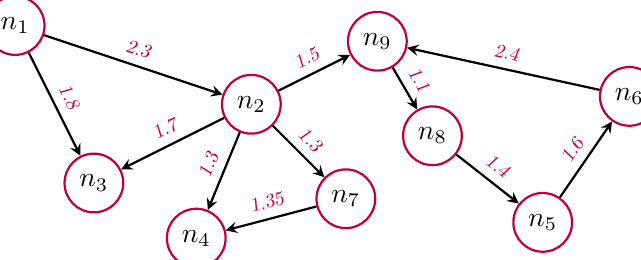
\begin{tikzpicture}[remember picture]
      \newcommand{\weight}[1]{node[midway,sloped,above] {\scalebox{0.7}{\textsl{\textcolor{purple}{#1}}}}}
      \tikzstyle{edge}  = [thick,>=stealth,draw=black]
      \tikzstyle{dedge} = [thick,->,>=stealth,draw=black]
      \tikzstyle{node}=[
        overlay,
        circle,
        draw=purple,
        anchor=center,
        thick,
        minimum size=1,
      ]
      
      \node[node] (n1) at (-4,0) {$n_1$};
      \node[node] (n2) at (-1,-1) {$n_2$};
      \node[node] (n3) at (-3,-2) {$n_3$};
      \node[node] (n4) at (-1.7,-2.7) {$n_4$};
      \node[node] (n5) at (2.7,-2.5) {$n_5$};
      \node[node] (n6) at (3.8,-0.9) {$n_6$};
      \node[node] (n7) at (0.2,-2.2) {$n_7$};
      \node[node] (n8) at (1.3,-1.4) {$n_8$};
      \node[node] (n9) at (0.6,-0.2) {$n_9$};
      
      \draw[dedge] (n1)--(n2) \weight{2.3};
      \draw[dedge] (n2)--(n3) \weight{1.7};
      \draw[dedge] (n1)--(n3) \weight{1.8};
      \draw[dedge] (n2)--(n4) \weight{1.3};
      \draw[dedge] (n2)--(n9) \weight{1.5};
      \draw[dedge] (n9)--(n8) \weight{1.1};
      \draw[dedge] (n6)--(n9) \weight{2.4};
      \draw[dedge] (n5)--(n6) \weight{1.6};
      \draw[dedge] (n2)--(n7) \weight{1.3};
      \draw[dedge] (n7)--(n4) \weight{1.35};
      \draw[dedge] (n8)--(n5) \weight{1.4};
    \end{tikzpicture}
  \end{center}
  \caption{Example of directed graph with weighted edges.}
  \label{fig:topics:graphs:example:base}
\end{figure}

\subsection{Paths}

\begin{figure}[tbp]
  \begin{center}
    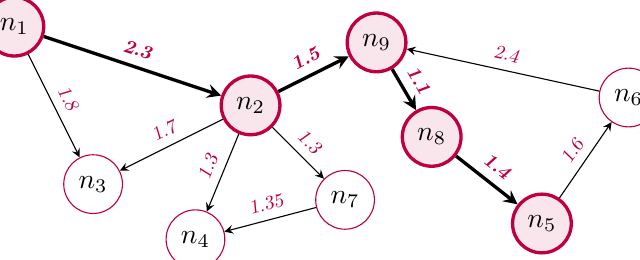
\begin{tikzpicture}[remember picture]
      \newcommand{\weight}[1]{node[midway,sloped,above] {\scalebox{0.7}{\textsl{\textcolor{purple}{#1}}}}}
      \tikzstyle{edge}  = [>=stealth,draw=black]
      \tikzstyle{dedge} = [->,>=stealth,draw=black]
      \tikzstyle{node}=[
        overlay,
        circle,
        draw=purple,
        anchor=center,
        minimum size=1,
      ]
      
      \node[node, very thick, fill=purple!10] (n1) at (-4,0) {$n_1$};
      \node[node, very thick, fill=purple!10] (n2) at (-1,-1) {$n_2$};
      \node[node] (n3) at (-3,-2) {$n_3$};
      \node[node] (n4) at (-1.7,-2.7) {$n_4$};
      \node[node, very thick, fill=purple!10] (n5) at (2.7,-2.5) {$n_5$};
      \node[node] (n6) at (3.8,-0.9) {$n_6$};
      \node[node] (n7) at (0.2,-2.2) {$n_7$};
      \node[node, very thick, fill=purple!10] (n8) at (1.3,-1.4) {$n_8$};
      \node[node, very thick, fill=purple!10] (n9) at (0.6,-0.2) {$n_9$};
      
      \draw[dedge, very thick] (n1)--(n2) \weight{\textbf{2.3}};
      \draw[dedge] (n2)--(n3) \weight{1.7};
      \draw[dedge] (n1)--(n3) \weight{1.8};
      \draw[dedge] (n2)--(n4) \weight{1.3};
      \draw[dedge, very thick] (n2)--(n9) \weight{\textbf{1.5}};
      \draw[dedge, very thick] (n9)--(n8) \weight{\textbf{1.1}};
      \draw[dedge] (n6)--(n9) \weight{2.4};
      \draw[dedge] (n5)--(n6) \weight{1.6};
      \draw[dedge] (n2)--(n7) \weight{1.3};
      \draw[dedge] (n7)--(n4) \weight{1.35};
      \draw[dedge, very thick] (n8)--(n5) \weight{\textbf{1.4}};
    \end{tikzpicture}
  \end{center}
  \caption[Example of a path in a directed graph.]{Example of a path in a directed graph. The path starts in $n_1$, goes through nodes $n_2$, $n_9$, $n_8$ to end in $n_5$. It has a total length of 6.3.}
  \label{fig:topics:graphs:example:path}
\end{figure}

\subsection{Cycles}

\begin{figure}[tbp]
  \begin{center}
    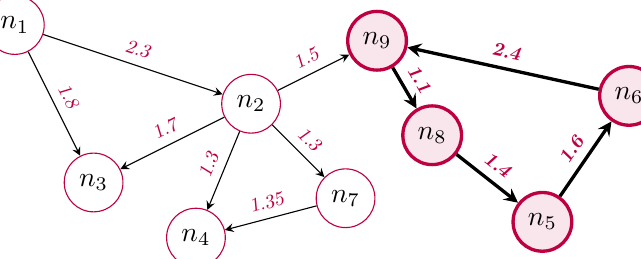
\begin{tikzpicture}[remember picture]
      \newcommand{\weight}[1]{node[midway,sloped,above] {\scalebox{0.7}{\textsl{\textcolor{purple}{#1}}}}}
      \tikzstyle{edge}  = [>=stealth,draw=black]
      \tikzstyle{dedge} = [->,>=stealth,draw=black]
      \tikzstyle{node}=[
        overlay,
        circle,
        draw=purple,
        anchor=center,
        minimum size=1,
      ]
      
      \node[node] (n1) at (-4,0) {$n_1$};
      \node[node] (n2) at (-1,-1) {$n_2$};
      \node[node] (n3) at (-3,-2) {$n_3$};
      \node[node] (n4) at (-1.7,-2.7) {$n_4$};
      \node[node, very thick, fill=purple!10] (n5) at (2.7,-2.5) {$n_5$};
      \node[node, very thick, fill=purple!10] (n6) at (3.8,-0.9) {$n_6$};
      \node[node] (n7) at (0.2,-2.2) {$n_7$};
      \node[node, very thick, fill=purple!10] (n8) at (1.3,-1.4) {$n_8$};
      \node[node, very thick, fill=purple!10] (n9) at (0.6,-0.2) {$n_9$};
      
      \draw[dedge] (n1)--(n2) \weight{2.3};
      \draw[dedge] (n2)--(n3) \weight{1.7};
      \draw[dedge] (n1)--(n3) \weight{1.8};
      \draw[dedge] (n2)--(n4) \weight{1.3};
      \draw[dedge] (n2)--(n9) \weight{1.5};
      \draw[dedge, very thick] (n9)--(n8) \weight{\textbf{1.1}};
      \draw[dedge, very thick] (n6)--(n9) \weight{\textbf{2.4}};
      \draw[dedge, very thick] (n5)--(n6) \weight{\textbf{1.6}};
      \draw[dedge] (n2)--(n7) \weight{1.3};
      \draw[dedge] (n7)--(n4) \weight{1.35};
      \draw[dedge, very thick] (n8)--(n5) \weight{\textbf{1.4}};
    \end{tikzpicture}
  \end{center}
  \caption[Example of a cycle in a directed graph.]{Example of a cycle in a directed graph. It goes through nodes $n_9$, $n_8$, $n_5$, and $n_6$.}
  
  \label{fig:topics:graphs:example:cycle}
\end{figure}

\subsection{Directed Acyclic Graphs}

\subsection{Trees}

\subsection{Connectedness}

\subsection{Reachability}

\subsection{Representation}
\subsubsection{Marshalling}

Graphs can be stored in many formats, but one of the more common ones is the DOT\footnote{ \url{https://en.wikipedia.org/wiki/DOT_\%28graph_description_language\%29} } file format.

\subsubsection{Datastructures}

\subsection{Property Graphs}

\subsection{Visual Layout}

\subsection{Use Cases}

\begin{itemize}
  \descitem{Filesystem}
  \descitem{GIT}
  \descitem{User Interfaces}
  \descitem{Dependency Modeling}
  \descitem{HTML/XML}
  \descitem{Route Planning}
  \descitem{Code Optimization}
\end{itemize}


\section{Algorithms}

\subsection{Backtracking}

\subsection{Sorting}

\subsubsection{Bubble Sort}
\subsubsection{Merge Sort}
\subsubsection{Quicksort}
\subsubsection{Radix Sort}

\subsection{Recursion}

\subsection{Misc}

\subsubsection{Levenshtein Distance}

\url{https://en.wikipedia.org/wiki/Levenshtein_distance}

\section{Algorithmic Complexity}

\subsection{Big O Notation}

\subsection{Amortized Cost}

\subsection{NP Completeness}


\section{State Machines}

\subsection{Parsing}

\subsection{Protocols}


\section{Scheduling}
\subsection{Cooperative Scheduling}

% def

\subsection{Preemptive Scheduling}

% def

% classical implementation

% granularity: timeslice


\section{Concurrency}
\subsection{Multiplexing}
\subsubsection{Fibers?}
\subsection{Threads}
\subsubsection{Kernel Threads}
\subsubsection{User Threads}
\subsection{Message Passing}


\section{Synchronization}
\subsection{Critical Sections}
\subsection{Mutexes}

\idx{Mutex}\url{https://en.wikipedia.org/wiki/Lock_(computer_science)}

\subsection{Semaphores}
\subsection{Monitors}
\subsection{Barriers}
\subsection{Wait Groups}


\section{FLow}
\subsection{Back Pressure}




\chapter{Topics}

\section{Graphs}

A graph\idx{Graph} is a structure that can be used to model how things relate to each other. Graphs consists of nodes\idx{Node} (also called vertices) and edges\idx{Edge} between them. There are many variations over the theme, but the most basic one is the \textsl{undirected}\idxx{Graph!Undirected}{Undirected} graph. It can be defined as:
\begin{eqnarray*}
  G = (N,E)
\end{eqnarray*}
Here, $N$ is the set of nodes and $E$ is the set of edges. We often choose to illustrate nodes as circles or boxes, and edges as lines.

% edges: directionality


\begin{figure}[tbp]
  \begin{center}
    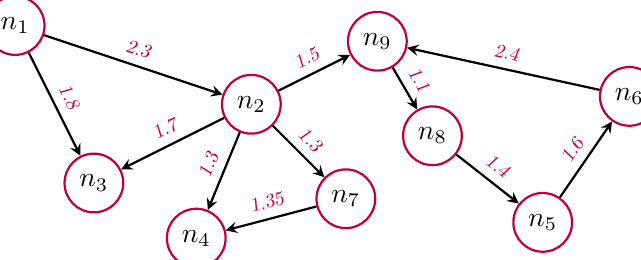
\begin{tikzpicture}[remember picture]
      \newcommand{\weight}[1]{node[midway,sloped,above] {\scalebox{0.7}{\textsl{\textcolor{purple}{#1}}}}}
      \tikzstyle{edge}  = [thick,>=stealth,draw=black]
      \tikzstyle{dedge} = [thick,->,>=stealth,draw=black]
      \tikzstyle{node}=[
        overlay,
        circle,
        draw=purple,
        anchor=center,
        thick,
        minimum size=1,
      ]
      
      \node[node] (n1) at (-4,0) {$n_1$};
      \node[node] (n2) at (-1,-1) {$n_2$};
      \node[node] (n3) at (-3,-2) {$n_3$};
      \node[node] (n4) at (-1.7,-2.7) {$n_4$};
      \node[node] (n5) at (2.7,-2.5) {$n_5$};
      \node[node] (n6) at (3.8,-0.9) {$n_6$};
      \node[node] (n7) at (0.2,-2.2) {$n_7$};
      \node[node] (n8) at (1.3,-1.4) {$n_8$};
      \node[node] (n9) at (0.6,-0.2) {$n_9$};
      
      \draw[dedge] (n1)--(n2) \weight{2.3};
      \draw[dedge] (n2)--(n3) \weight{1.7};
      \draw[dedge] (n1)--(n3) \weight{1.8};
      \draw[dedge] (n2)--(n4) \weight{1.3};
      \draw[dedge] (n2)--(n9) \weight{1.5};
      \draw[dedge] (n9)--(n8) \weight{1.1};
      \draw[dedge] (n6)--(n9) \weight{2.4};
      \draw[dedge] (n5)--(n6) \weight{1.6};
      \draw[dedge] (n2)--(n7) \weight{1.3};
      \draw[dedge] (n7)--(n4) \weight{1.35};
      \draw[dedge] (n8)--(n5) \weight{1.4};
    \end{tikzpicture}
  \end{center}
  \caption{Example of directed graph with weighted edges.}
  \label{fig:topics:graphs:example:base}
\end{figure}

\subsection{Paths}

\begin{figure}[tbp]
  \begin{center}
    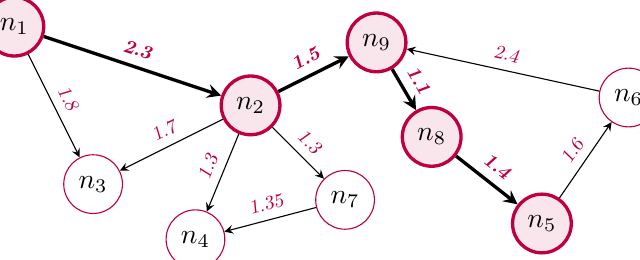
\begin{tikzpicture}[remember picture]
      \newcommand{\weight}[1]{node[midway,sloped,above] {\scalebox{0.7}{\textsl{\textcolor{purple}{#1}}}}}
      \tikzstyle{edge}  = [>=stealth,draw=black]
      \tikzstyle{dedge} = [->,>=stealth,draw=black]
      \tikzstyle{node}=[
        overlay,
        circle,
        draw=purple,
        anchor=center,
        minimum size=1,
      ]
      
      \node[node, very thick, fill=purple!10] (n1) at (-4,0) {$n_1$};
      \node[node, very thick, fill=purple!10] (n2) at (-1,-1) {$n_2$};
      \node[node] (n3) at (-3,-2) {$n_3$};
      \node[node] (n4) at (-1.7,-2.7) {$n_4$};
      \node[node, very thick, fill=purple!10] (n5) at (2.7,-2.5) {$n_5$};
      \node[node] (n6) at (3.8,-0.9) {$n_6$};
      \node[node] (n7) at (0.2,-2.2) {$n_7$};
      \node[node, very thick, fill=purple!10] (n8) at (1.3,-1.4) {$n_8$};
      \node[node, very thick, fill=purple!10] (n9) at (0.6,-0.2) {$n_9$};
      
      \draw[dedge, very thick] (n1)--(n2) \weight{\textbf{2.3}};
      \draw[dedge] (n2)--(n3) \weight{1.7};
      \draw[dedge] (n1)--(n3) \weight{1.8};
      \draw[dedge] (n2)--(n4) \weight{1.3};
      \draw[dedge, very thick] (n2)--(n9) \weight{\textbf{1.5}};
      \draw[dedge, very thick] (n9)--(n8) \weight{\textbf{1.1}};
      \draw[dedge] (n6)--(n9) \weight{2.4};
      \draw[dedge] (n5)--(n6) \weight{1.6};
      \draw[dedge] (n2)--(n7) \weight{1.3};
      \draw[dedge] (n7)--(n4) \weight{1.35};
      \draw[dedge, very thick] (n8)--(n5) \weight{\textbf{1.4}};
    \end{tikzpicture}
  \end{center}
  \caption[Example of a path in a directed graph.]{Example of a path in a directed graph. The path starts in $n_1$, goes through nodes $n_2$, $n_9$, $n_8$ to end in $n_5$. It has a total length of 6.3.}
  \label{fig:topics:graphs:example:path}
\end{figure}

\subsection{Cycles}

\begin{figure}[tbp]
  \begin{center}
    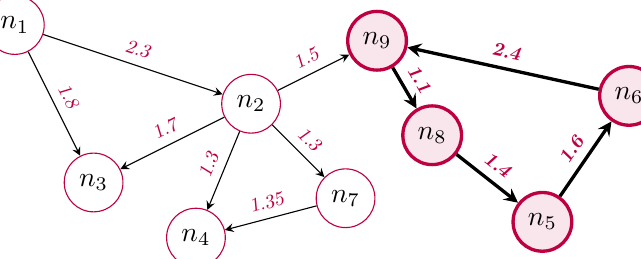
\begin{tikzpicture}[remember picture]
      \newcommand{\weight}[1]{node[midway,sloped,above] {\scalebox{0.7}{\textsl{\textcolor{purple}{#1}}}}}
      \tikzstyle{edge}  = [>=stealth,draw=black]
      \tikzstyle{dedge} = [->,>=stealth,draw=black]
      \tikzstyle{node}=[
        overlay,
        circle,
        draw=purple,
        anchor=center,
        minimum size=1,
      ]
      
      \node[node] (n1) at (-4,0) {$n_1$};
      \node[node] (n2) at (-1,-1) {$n_2$};
      \node[node] (n3) at (-3,-2) {$n_3$};
      \node[node] (n4) at (-1.7,-2.7) {$n_4$};
      \node[node, very thick, fill=purple!10] (n5) at (2.7,-2.5) {$n_5$};
      \node[node, very thick, fill=purple!10] (n6) at (3.8,-0.9) {$n_6$};
      \node[node] (n7) at (0.2,-2.2) {$n_7$};
      \node[node, very thick, fill=purple!10] (n8) at (1.3,-1.4) {$n_8$};
      \node[node, very thick, fill=purple!10] (n9) at (0.6,-0.2) {$n_9$};
      
      \draw[dedge] (n1)--(n2) \weight{2.3};
      \draw[dedge] (n2)--(n3) \weight{1.7};
      \draw[dedge] (n1)--(n3) \weight{1.8};
      \draw[dedge] (n2)--(n4) \weight{1.3};
      \draw[dedge] (n2)--(n9) \weight{1.5};
      \draw[dedge, very thick] (n9)--(n8) \weight{\textbf{1.1}};
      \draw[dedge, very thick] (n6)--(n9) \weight{\textbf{2.4}};
      \draw[dedge, very thick] (n5)--(n6) \weight{\textbf{1.6}};
      \draw[dedge] (n2)--(n7) \weight{1.3};
      \draw[dedge] (n7)--(n4) \weight{1.35};
      \draw[dedge, very thick] (n8)--(n5) \weight{\textbf{1.4}};
    \end{tikzpicture}
  \end{center}
  \caption[Example of a cycle in a directed graph.]{Example of a cycle in a directed graph. It goes through nodes $n_9$, $n_8$, $n_5$, and $n_6$.}
  
  \label{fig:topics:graphs:example:cycle}
\end{figure}

\subsection{Directed Acyclic Graphs}

\subsection{Trees}

\subsection{Connectedness}

\subsection{Reachability}

\subsection{Representation}
\subsubsection{Marshalling}

Graphs can be stored in many formats, but one of the more common ones is the DOT\footnote{ \url{https://en.wikipedia.org/wiki/DOT_\%28graph_description_language\%29} } file format.

\subsubsection{Datastructures}

\subsection{Property Graphs}

\subsection{Visual Layout}

\subsection{Use Cases}

\begin{itemize}
  \descitem{Filesystem}
  \descitem{GIT}
  \descitem{User Interfaces}
  \descitem{Dependency Modeling}
  \descitem{HTML/XML}
  \descitem{Route Planning}
  \descitem{Code Optimization}
\end{itemize}


\section{Algorithms}

\subsection{Backtracking}

\subsection{Sorting}

\subsubsection{Bubble Sort}
\subsubsection{Merge Sort}
\subsubsection{Quicksort}
\subsubsection{Radix Sort}

\subsection{Recursion}

\subsection{Misc}

\subsubsection{Levenshtein Distance}

\url{https://en.wikipedia.org/wiki/Levenshtein_distance}

\section{Algorithmic Complexity}

\subsection{Big O Notation}

\subsection{Amortized Cost}

\subsection{NP Completeness}


\section{State Machines}

\subsection{Parsing}

\subsection{Protocols}


\section{Scheduling}
\subsection{Cooperative Scheduling}

% def

\subsection{Preemptive Scheduling}

% def

% classical implementation

% granularity: timeslice


\section{Concurrency}
\subsection{Multiplexing}
\subsubsection{Fibers?}
\subsection{Threads}
\subsubsection{Kernel Threads}
\subsubsection{User Threads}
\subsection{Message Passing}


\section{Synchronization}
\subsection{Critical Sections}
\subsection{Mutexes}

\idx{Mutex}\url{https://en.wikipedia.org/wiki/Lock_(computer_science)}

\subsection{Semaphores}
\subsection{Monitors}
\subsection{Barriers}
\subsection{Wait Groups}


\section{FLow}
\subsection{Back Pressure}




\chapter{Topics}

\section{Graphs}

A graph\idx{Graph} is a structure that can be used to model how things relate to each other. Graphs consists of nodes\idx{Node} (also called vertices) and edges\idx{Edge} between them. There are many variations over the theme, but the most basic one is the \textsl{undirected}\idxx{Graph!Undirected}{Undirected} graph. It can be defined as:
\begin{eqnarray*}
  G = (N,E)
\end{eqnarray*}
Here, $N$ is the set of nodes and $E$ is the set of edges. We often choose to illustrate nodes as circles or boxes, and edges as lines.

% edges: directionality


\begin{figure}[tbp]
  \begin{center}
    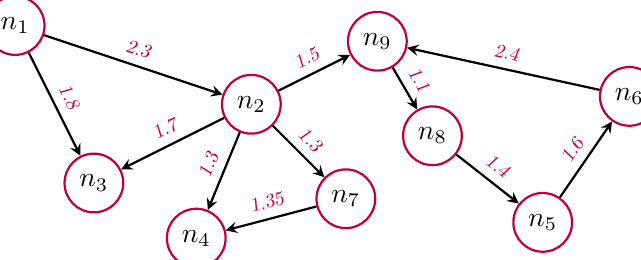
\begin{tikzpicture}[remember picture]
      \newcommand{\weight}[1]{node[midway,sloped,above] {\scalebox{0.7}{\textsl{\textcolor{purple}{#1}}}}}
      \tikzstyle{edge}  = [thick,>=stealth,draw=black]
      \tikzstyle{dedge} = [thick,->,>=stealth,draw=black]
      \tikzstyle{node}=[
        overlay,
        circle,
        draw=purple,
        anchor=center,
        thick,
        minimum size=1,
      ]
      
      \node[node] (n1) at (-4,0) {$n_1$};
      \node[node] (n2) at (-1,-1) {$n_2$};
      \node[node] (n3) at (-3,-2) {$n_3$};
      \node[node] (n4) at (-1.7,-2.7) {$n_4$};
      \node[node] (n5) at (2.7,-2.5) {$n_5$};
      \node[node] (n6) at (3.8,-0.9) {$n_6$};
      \node[node] (n7) at (0.2,-2.2) {$n_7$};
      \node[node] (n8) at (1.3,-1.4) {$n_8$};
      \node[node] (n9) at (0.6,-0.2) {$n_9$};
      
      \draw[dedge] (n1)--(n2) \weight{2.3};
      \draw[dedge] (n2)--(n3) \weight{1.7};
      \draw[dedge] (n1)--(n3) \weight{1.8};
      \draw[dedge] (n2)--(n4) \weight{1.3};
      \draw[dedge] (n2)--(n9) \weight{1.5};
      \draw[dedge] (n9)--(n8) \weight{1.1};
      \draw[dedge] (n6)--(n9) \weight{2.4};
      \draw[dedge] (n5)--(n6) \weight{1.6};
      \draw[dedge] (n2)--(n7) \weight{1.3};
      \draw[dedge] (n7)--(n4) \weight{1.35};
      \draw[dedge] (n8)--(n5) \weight{1.4};
    \end{tikzpicture}
  \end{center}
  \caption{Example of directed graph with weighted edges.}
  \label{fig:topics:graphs:example:base}
\end{figure}

\subsection{Paths}

\begin{figure}[tbp]
  \begin{center}
    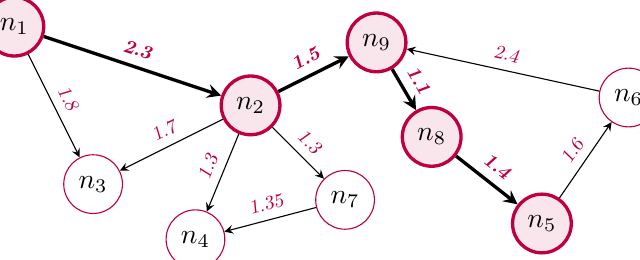
\begin{tikzpicture}[remember picture]
      \newcommand{\weight}[1]{node[midway,sloped,above] {\scalebox{0.7}{\textsl{\textcolor{purple}{#1}}}}}
      \tikzstyle{edge}  = [>=stealth,draw=black]
      \tikzstyle{dedge} = [->,>=stealth,draw=black]
      \tikzstyle{node}=[
        overlay,
        circle,
        draw=purple,
        anchor=center,
        minimum size=1,
      ]
      
      \node[node, very thick, fill=purple!10] (n1) at (-4,0) {$n_1$};
      \node[node, very thick, fill=purple!10] (n2) at (-1,-1) {$n_2$};
      \node[node] (n3) at (-3,-2) {$n_3$};
      \node[node] (n4) at (-1.7,-2.7) {$n_4$};
      \node[node, very thick, fill=purple!10] (n5) at (2.7,-2.5) {$n_5$};
      \node[node] (n6) at (3.8,-0.9) {$n_6$};
      \node[node] (n7) at (0.2,-2.2) {$n_7$};
      \node[node, very thick, fill=purple!10] (n8) at (1.3,-1.4) {$n_8$};
      \node[node, very thick, fill=purple!10] (n9) at (0.6,-0.2) {$n_9$};
      
      \draw[dedge, very thick] (n1)--(n2) \weight{\textbf{2.3}};
      \draw[dedge] (n2)--(n3) \weight{1.7};
      \draw[dedge] (n1)--(n3) \weight{1.8};
      \draw[dedge] (n2)--(n4) \weight{1.3};
      \draw[dedge, very thick] (n2)--(n9) \weight{\textbf{1.5}};
      \draw[dedge, very thick] (n9)--(n8) \weight{\textbf{1.1}};
      \draw[dedge] (n6)--(n9) \weight{2.4};
      \draw[dedge] (n5)--(n6) \weight{1.6};
      \draw[dedge] (n2)--(n7) \weight{1.3};
      \draw[dedge] (n7)--(n4) \weight{1.35};
      \draw[dedge, very thick] (n8)--(n5) \weight{\textbf{1.4}};
    \end{tikzpicture}
  \end{center}
  \caption[Example of a path in a directed graph.]{Example of a path in a directed graph. The path starts in $n_1$, goes through nodes $n_2$, $n_9$, $n_8$ to end in $n_5$. It has a total length of 6.3.}
  \label{fig:topics:graphs:example:path}
\end{figure}

\subsection{Cycles}

\begin{figure}[tbp]
  \begin{center}
    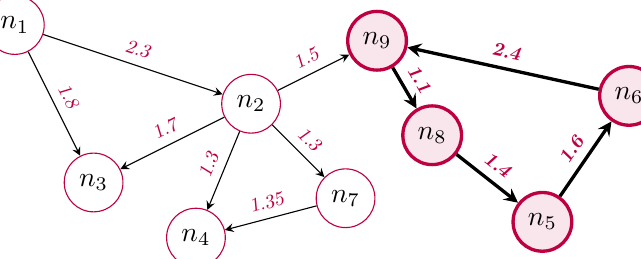
\begin{tikzpicture}[remember picture]
      \newcommand{\weight}[1]{node[midway,sloped,above] {\scalebox{0.7}{\textsl{\textcolor{purple}{#1}}}}}
      \tikzstyle{edge}  = [>=stealth,draw=black]
      \tikzstyle{dedge} = [->,>=stealth,draw=black]
      \tikzstyle{node}=[
        overlay,
        circle,
        draw=purple,
        anchor=center,
        minimum size=1,
      ]
      
      \node[node] (n1) at (-4,0) {$n_1$};
      \node[node] (n2) at (-1,-1) {$n_2$};
      \node[node] (n3) at (-3,-2) {$n_3$};
      \node[node] (n4) at (-1.7,-2.7) {$n_4$};
      \node[node, very thick, fill=purple!10] (n5) at (2.7,-2.5) {$n_5$};
      \node[node, very thick, fill=purple!10] (n6) at (3.8,-0.9) {$n_6$};
      \node[node] (n7) at (0.2,-2.2) {$n_7$};
      \node[node, very thick, fill=purple!10] (n8) at (1.3,-1.4) {$n_8$};
      \node[node, very thick, fill=purple!10] (n9) at (0.6,-0.2) {$n_9$};
      
      \draw[dedge] (n1)--(n2) \weight{2.3};
      \draw[dedge] (n2)--(n3) \weight{1.7};
      \draw[dedge] (n1)--(n3) \weight{1.8};
      \draw[dedge] (n2)--(n4) \weight{1.3};
      \draw[dedge] (n2)--(n9) \weight{1.5};
      \draw[dedge, very thick] (n9)--(n8) \weight{\textbf{1.1}};
      \draw[dedge, very thick] (n6)--(n9) \weight{\textbf{2.4}};
      \draw[dedge, very thick] (n5)--(n6) \weight{\textbf{1.6}};
      \draw[dedge] (n2)--(n7) \weight{1.3};
      \draw[dedge] (n7)--(n4) \weight{1.35};
      \draw[dedge, very thick] (n8)--(n5) \weight{\textbf{1.4}};
    \end{tikzpicture}
  \end{center}
  \caption[Example of a cycle in a directed graph.]{Example of a cycle in a directed graph. It goes through nodes $n_9$, $n_8$, $n_5$, and $n_6$.}
  
  \label{fig:topics:graphs:example:cycle}
\end{figure}

\subsection{Directed Acyclic Graphs}

\subsection{Trees}

\subsection{Connectedness}

\subsection{Reachability}

\subsection{Representation}
\subsubsection{Marshalling}

Graphs can be stored in many formats, but one of the more common ones is the DOT\footnote{ \url{https://en.wikipedia.org/wiki/DOT_\%28graph_description_language\%29} } file format.

\subsubsection{Datastructures}

\subsection{Property Graphs}

\subsection{Visual Layout}

\subsection{Use Cases}

\begin{itemize}
  \descitem{Filesystem}
  \descitem{GIT}
  \descitem{User Interfaces}
  \descitem{Dependency Modeling}
  \descitem{HTML/XML}
  \descitem{Route Planning}
  \descitem{Code Optimization}
\end{itemize}


\section{Algorithms}

\subsection{Backtracking}

\subsection{Sorting}

\subsubsection{Bubble Sort}
\subsubsection{Merge Sort}
\subsubsection{Quicksort}
\subsubsection{Radix Sort}

\subsection{Recursion}

\subsection{Misc}

\subsubsection{Levenshtein Distance}

\url{https://en.wikipedia.org/wiki/Levenshtein_distance}

\section{Algorithmic Complexity}

\subsection{Big O Notation}

\subsection{Amortized Cost}

\subsection{NP Completeness}


\section{State Machines}

\subsection{Parsing}

\subsection{Protocols}


\section{Scheduling}
\subsection{Cooperative Scheduling}

% def

\subsection{Preemptive Scheduling}

% def

% classical implementation

% granularity: timeslice


\section{Concurrency}
\subsection{Multiplexing}
\subsubsection{Fibers?}
\subsection{Threads}
\subsubsection{Kernel Threads}
\subsubsection{User Threads}
\subsection{Message Passing}


\section{Synchronization}
\subsection{Critical Sections}
\subsection{Mutexes}

\idx{Mutex}\url{https://en.wikipedia.org/wiki/Lock_(computer_science)}

\subsection{Semaphores}
\subsection{Monitors}
\subsection{Barriers}
\subsection{Wait Groups}


\section{FLow}
\subsection{Back Pressure}




\chapter{Topics}

\section{Graphs}

A graph\idx{Graph} is a structure that can be used to model how things relate to each other. Graphs consists of nodes\idx{Node} (also called vertices) and edges\idx{Edge} between them. There are many variations over the theme, but the most basic one is the \textsl{undirected}\idxx{Graph!Undirected}{Undirected} graph. It can be defined as:
\begin{eqnarray*}
  G = (N,E)
\end{eqnarray*}
Here, $N$ is the set of nodes and $E$ is the set of edges. We often choose to illustrate nodes as circles or boxes, and edges as lines.

% edges: directionality


\begin{figure}[tbp]
  \begin{center}
    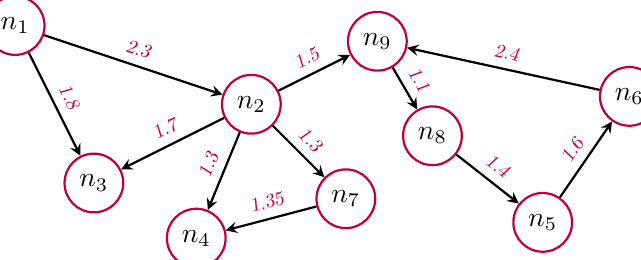
\begin{tikzpicture}[remember picture]
      \newcommand{\weight}[1]{node[midway,sloped,above] {\scalebox{0.7}{\textsl{\textcolor{purple}{#1}}}}}
      \tikzstyle{edge}  = [thick,>=stealth,draw=black]
      \tikzstyle{dedge} = [thick,->,>=stealth,draw=black]
      \tikzstyle{node}=[
        overlay,
        circle,
        draw=purple,
        anchor=center,
        thick,
        minimum size=1,
      ]
      
      \node[node] (n1) at (-4,0) {$n_1$};
      \node[node] (n2) at (-1,-1) {$n_2$};
      \node[node] (n3) at (-3,-2) {$n_3$};
      \node[node] (n4) at (-1.7,-2.7) {$n_4$};
      \node[node] (n5) at (2.7,-2.5) {$n_5$};
      \node[node] (n6) at (3.8,-0.9) {$n_6$};
      \node[node] (n7) at (0.2,-2.2) {$n_7$};
      \node[node] (n8) at (1.3,-1.4) {$n_8$};
      \node[node] (n9) at (0.6,-0.2) {$n_9$};
      
      \draw[dedge] (n1)--(n2) \weight{2.3};
      \draw[dedge] (n2)--(n3) \weight{1.7};
      \draw[dedge] (n1)--(n3) \weight{1.8};
      \draw[dedge] (n2)--(n4) \weight{1.3};
      \draw[dedge] (n2)--(n9) \weight{1.5};
      \draw[dedge] (n9)--(n8) \weight{1.1};
      \draw[dedge] (n6)--(n9) \weight{2.4};
      \draw[dedge] (n5)--(n6) \weight{1.6};
      \draw[dedge] (n2)--(n7) \weight{1.3};
      \draw[dedge] (n7)--(n4) \weight{1.35};
      \draw[dedge] (n8)--(n5) \weight{1.4};
    \end{tikzpicture}
  \end{center}
  \caption{Example of directed graph with weighted edges.}
  \label{fig:topics:graphs:example:base}
\end{figure}

\subsection{Paths}

\begin{figure}[tbp]
  \begin{center}
    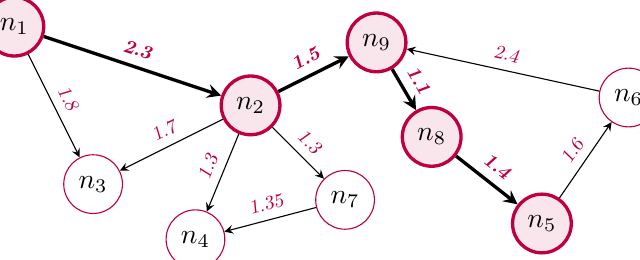
\begin{tikzpicture}[remember picture]
      \newcommand{\weight}[1]{node[midway,sloped,above] {\scalebox{0.7}{\textsl{\textcolor{purple}{#1}}}}}
      \tikzstyle{edge}  = [>=stealth,draw=black]
      \tikzstyle{dedge} = [->,>=stealth,draw=black]
      \tikzstyle{node}=[
        overlay,
        circle,
        draw=purple,
        anchor=center,
        minimum size=1,
      ]
      
      \node[node, very thick, fill=purple!10] (n1) at (-4,0) {$n_1$};
      \node[node, very thick, fill=purple!10] (n2) at (-1,-1) {$n_2$};
      \node[node] (n3) at (-3,-2) {$n_3$};
      \node[node] (n4) at (-1.7,-2.7) {$n_4$};
      \node[node, very thick, fill=purple!10] (n5) at (2.7,-2.5) {$n_5$};
      \node[node] (n6) at (3.8,-0.9) {$n_6$};
      \node[node] (n7) at (0.2,-2.2) {$n_7$};
      \node[node, very thick, fill=purple!10] (n8) at (1.3,-1.4) {$n_8$};
      \node[node, very thick, fill=purple!10] (n9) at (0.6,-0.2) {$n_9$};
      
      \draw[dedge, very thick] (n1)--(n2) \weight{\textbf{2.3}};
      \draw[dedge] (n2)--(n3) \weight{1.7};
      \draw[dedge] (n1)--(n3) \weight{1.8};
      \draw[dedge] (n2)--(n4) \weight{1.3};
      \draw[dedge, very thick] (n2)--(n9) \weight{\textbf{1.5}};
      \draw[dedge, very thick] (n9)--(n8) \weight{\textbf{1.1}};
      \draw[dedge] (n6)--(n9) \weight{2.4};
      \draw[dedge] (n5)--(n6) \weight{1.6};
      \draw[dedge] (n2)--(n7) \weight{1.3};
      \draw[dedge] (n7)--(n4) \weight{1.35};
      \draw[dedge, very thick] (n8)--(n5) \weight{\textbf{1.4}};
    \end{tikzpicture}
  \end{center}
  \caption[Example of a path in a directed graph.]{Example of a path in a directed graph. The path starts in $n_1$, goes through nodes $n_2$, $n_9$, $n_8$ to end in $n_5$. It has a total length of 6.3.}
  \label{fig:topics:graphs:example:path}
\end{figure}

\subsection{Cycles}

\begin{figure}[tbp]
  \begin{center}
    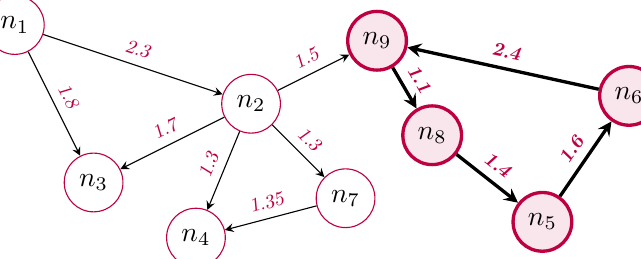
\begin{tikzpicture}[remember picture]
      \newcommand{\weight}[1]{node[midway,sloped,above] {\scalebox{0.7}{\textsl{\textcolor{purple}{#1}}}}}
      \tikzstyle{edge}  = [>=stealth,draw=black]
      \tikzstyle{dedge} = [->,>=stealth,draw=black]
      \tikzstyle{node}=[
        overlay,
        circle,
        draw=purple,
        anchor=center,
        minimum size=1,
      ]
      
      \node[node] (n1) at (-4,0) {$n_1$};
      \node[node] (n2) at (-1,-1) {$n_2$};
      \node[node] (n3) at (-3,-2) {$n_3$};
      \node[node] (n4) at (-1.7,-2.7) {$n_4$};
      \node[node, very thick, fill=purple!10] (n5) at (2.7,-2.5) {$n_5$};
      \node[node, very thick, fill=purple!10] (n6) at (3.8,-0.9) {$n_6$};
      \node[node] (n7) at (0.2,-2.2) {$n_7$};
      \node[node, very thick, fill=purple!10] (n8) at (1.3,-1.4) {$n_8$};
      \node[node, very thick, fill=purple!10] (n9) at (0.6,-0.2) {$n_9$};
      
      \draw[dedge] (n1)--(n2) \weight{2.3};
      \draw[dedge] (n2)--(n3) \weight{1.7};
      \draw[dedge] (n1)--(n3) \weight{1.8};
      \draw[dedge] (n2)--(n4) \weight{1.3};
      \draw[dedge] (n2)--(n9) \weight{1.5};
      \draw[dedge, very thick] (n9)--(n8) \weight{\textbf{1.1}};
      \draw[dedge, very thick] (n6)--(n9) \weight{\textbf{2.4}};
      \draw[dedge, very thick] (n5)--(n6) \weight{\textbf{1.6}};
      \draw[dedge] (n2)--(n7) \weight{1.3};
      \draw[dedge] (n7)--(n4) \weight{1.35};
      \draw[dedge, very thick] (n8)--(n5) \weight{\textbf{1.4}};
    \end{tikzpicture}
  \end{center}
  \caption[Example of a cycle in a directed graph.]{Example of a cycle in a directed graph. It goes through nodes $n_9$, $n_8$, $n_5$, and $n_6$.}
  
  \label{fig:topics:graphs:example:cycle}
\end{figure}

\subsection{Directed Acyclic Graphs}

\subsection{Trees}

\subsection{Connectedness}

\subsection{Reachability}

\subsection{Representation}
\subsubsection{Marshalling}

Graphs can be stored in many formats, but one of the more common ones is the DOT\footnote{ \url{https://en.wikipedia.org/wiki/DOT_\%28graph_description_language\%29} } file format.

\subsubsection{Datastructures}

\subsection{Property Graphs}

\subsection{Visual Layout}

\subsection{Use Cases}

\begin{itemize}
  \descitem{Filesystem}
  \descitem{GIT}
  \descitem{User Interfaces}
  \descitem{Dependency Modeling}
  \descitem{HTML/XML}
  \descitem{Route Planning}
  \descitem{Code Optimization}
\end{itemize}


\section{Algorithms}

\subsection{Backtracking}

\subsection{Sorting}

\subsubsection{Bubble Sort}
\subsubsection{Merge Sort}
\subsubsection{Quicksort}
\subsubsection{Radix Sort}

\subsection{Recursion}

\subsection{Misc}

\subsubsection{Levenshtein Distance}

\url{https://en.wikipedia.org/wiki/Levenshtein_distance}

\section{Algorithmic Complexity}

\subsection{Big O Notation}

\subsection{Amortized Cost}

\subsection{NP Completeness}


\section{State Machines}

\subsection{Parsing}

\subsection{Protocols}


\section{Scheduling}
\subsection{Cooperative Scheduling}

% def

\subsection{Preemptive Scheduling}

% def

% classical implementation

% granularity: timeslice


\section{Concurrency}
\subsection{Multiplexing}
\subsubsection{Fibers?}
\subsection{Threads}
\subsubsection{Kernel Threads}
\subsubsection{User Threads}
\subsection{Message Passing}


\section{Synchronization}
\subsection{Critical Sections}
\subsection{Mutexes}

\idx{Mutex}\url{https://en.wikipedia.org/wiki/Lock_(computer_science)}

\subsection{Semaphores}
\subsection{Monitors}
\subsection{Barriers}
\subsection{Wait Groups}


\section{FLow}
\subsection{Back Pressure}





\printbibliography

\printindex

\end{document}
